%Package Date: 2018-01-01 % !TeX program = XeLaTeX

\documentclass[12pt]{report} \usepackage{preamble}

\title{\textbf{\huge Vulkan Unveiled: A Beginner's Guide to Professional
Graphics Programming}} \author {Nick Schefner}
\bibliography{citations.bib}

\begin{document} \maketitle

\tableofcontents

\chapter{Introduction}

Dear Reader,

Welcome to "Vulkan Unveiled: A Beginner's Guide to Professional Graphics Programming".
It is with great pleasure and excitement that I extend my sincerest greetings
to you as you embark on this journey into the world of Vulkan API.
Before we start, I would like to introduce myself to you.

I began my journey with the Vulkan API about 3 months ago when I embarked
on the creation of my own game engine “Magma”, which is just a very basic
implementation of a game engine. Before that, I have
started my programming journey with the well known Unity Game Engine
and learned many basics on how games and graphics behave. I also have
experience with Glium, which is an OpenGL Wrapper for Rust. For those
unfamiliar, Glium further abstracts OpenGL, which made it easier to
understand the logic and functionalities of my application.  I’m deeply
invested in creating a precise representation of the Vulkan API.
Which will also be my ground base on further deepening my knowledge and
understanding.	While researching and writing this book, I anticipate
learning a great deal myself.  Nonetheless, I am committed to providing
you with a comprehensive understanding of graphics programming throughout
this book.

Graphical programming is a complex topic with a steep learning curve,
I often feel that I missed the dots connecting every aspect of the
underlying technologies when first getting started in this field as a
game dev. Therefore it might be quite overwhelming at first, to understand
how the graphics that we see every day are created and displayed onto
our displays. It does not help that Vulkan expands on that complexity
and provides us with an API that is very low level, whereas older graphic
APIs abstract many of the processes, that Vulkan requires us to handle
ourself.

Because Vulkan requires us to explicitly control the hardware resources,
you need even more knowledge about the multiple hardware components and
rendering possibilities that modern GPUs allow us to employ.

The main idea off this book is to slowly introduce someone who has had
no contact with graphical programming so far, but is excited to dive
into an interesting topic that is a must know for every aspiring future
game developer or artist. We will first learn to understand the GPU and
its usage. I will then focus on explaining pipelines, buffers, swap chains
and other components of the render system and explain in detail how they work
and are linked together. Besides that I will explain how Vulkan manages
each of these components and give an example on how a possible implementation
could look like.

I also want to give a special thanks to Brendan Galea for his “Vulkan
(c++) Game Engine” series, that helped me out a lot on understanding
not just Vulkan as an API but also the basics of graphical programming
and its components.

Lastly, I want to assure you that while learning Vulkan may seem daunting
at first, with time and patience, anyone interested in this topic can
develop a strong understanding of it.

\chapter{The GPU}

\section{Why do we need a GPU?}

The graphics processing unit (GPU) is, like the name implies, a hardware
component that is made specifically for processing graphical data. Sure,
okay, but why do we need a separate hardware component for that?  Why not
just let the CPU handle the calculations? The answer is simple: speed
and parallelism.

The CPU is great at executing one command after another, but
it is not very good at executing multiple commands at the same
time. Sure we have multi threading but the CPU is limited to just a
few cores. \cite{CDW-cpu_vs_gpu} On the other hand, the GPU is mainly
build on processing mathematically complex operations like matrix
multiplications, that are not just executed once but multiple
times. \cite{NVIDIA-cpu-gpu} Because the GPU focuses on speed
and parallelism, it is designed to use more of the accessible
transistors for processing data. This is beneficial for parallel
computations because the GPU can hide memory access latencies with
computation. The CPU on the other hand has an additional cache layer
and a more complex control logic that makes sequential computations
faster. \cite{CUDA_Programming_Guide}

Imagine creating a animation where the color of your full screen changes
between red and green. In that case you have a single command, the color
change, which is performed on every pixel on the screen. Using a CPU
we would have to wait for the CPU to execute the command on every pixel
one after another, which would take a lot of time. With the GPU we can
execute the command on every pixel simultaneously, which is much faster.

While a CPU usually just has a hand full of cores, GPUs have multiple
thousands of cores. \cite{NVIDIA-rtx-4090}
But that doesn't mean that the GPU is 1000
times faster than the CPU. The compute units of the GPU are much slower
than the cores of the CPU, but because they can run in parallel they are
more suitable for graphical computations. \cite{CUDA_Programming_Guide}

The GPU also has its own memory called the video random access memory
(VRAM) which is used to store processed and unprocessed data.
I don't want to go into detail about the VRAM because it is not relevant
for understanding Vulkan, but it is important to add that the VRAM
allows simultaneously reading and writing data, which is a big advantage
over the CPU. \cite{vram}

It might also be interesting that when the VRAM is full, rendering
speed and performance will drop because we need to get the data from a
slower memory source like the DRAM.  Therefore it is important to manage
data efficiently and to not overload the VRAM by, for example, loading
to many or to detailed textures.

\section{Basic Architecture of the GPU}

I've already mentioned that the GPU can take one instruction and
execute it on multiple threads at the same time. This is called SIMD
(Single Instruction, Multiple Data). \cite{cherry_gpu_architecture}

The GPU is made up of thousands of small cores, which are called CUDA
compute units on NVIDIA graphics cards \cite{CUDA_Programming_Guide}
and ROCm compute units on AMD graphics, which I will neglect to
simplify this topic. \cite{rocm} CUDA stands for "Compute Unified
Device Architecture" and is a low level parallel computing platform
and programming model that comes with an API for writing programs
that can handle the power and advantages of the GPU in a high level
language like c or c++. \cite{CUDA_Programming_Guide} Don't worry, we
will not use CUDA or an assembly language in this book, because Vulkan
abstracts the usage of the GPU for us, but it is important to understand
that the GPU is not just a black box that we can throw commands at and
expect it to work. These cores are combined into an array of so called
streaming multiprocessors (SM) also known as CUDA blocks, which are the
main building blocks of the GPU.  Each SM has its own control logic,
memory and execution units. \cite{CUDA_Programming_Guide} These SMs are
then combined into a grid called the GPU.  When the GPU is invoked by
the CPU, a free SM will be assigned to performing the requested tasks
and then return the results to the CPU if needed. \cite{CUDA_Programming_Guide}

The GPU also consists of a memory hierarchy, which is used to store the
data that is processed by the GPU. The memory hierarchy looks like this:

\begin{figure}[hbtp]
	\centering
	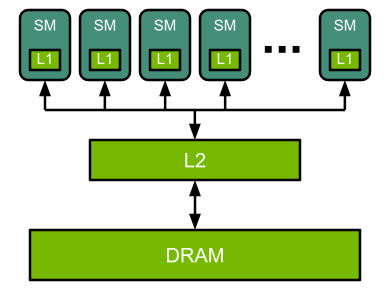
\includegraphics[width=0.70\textwidth]{simple-gpu-arch.png}
	\caption{Memory Hierarchy of the GPU \cite{fig:gpu-arch}}
\end{figure}

Please note that the VRAM is not part of the memory hierarchy, but is
connected to the L2 cache. Caches are used to store frequently used
data and to reduce access times to the main memory. While every SM
has its own L1 cache, the L2 cache is shared between all SMs. Which
means that all cores in one SM are sharing one L1 cache. The CPU
on the other hand has one cache and one memory controller per
core. \cite{CUDA_Programming_Guide}

\section {Summary}

Okay that was a lot of information, so let's summarize the really
important bits of what we have learned so far.

The GPU was created to process graphical data much faster than a CPU
could ever do. It allows us to execute the same command on multiple
data simultaneously to prevent waiting for a single command to finish,
which helps us render reoccurring tasks like drawing a texture or model
much faster.  It is made up of many cores which are combined into an
array of streaming multiprocessors (SM) to allow better control and
management of the cores.  The VRAM is the memory of the GPU and its
important to optimize your data to prevent overloading the VRAM.

\chapter{Graphics Rendering Pipeline}

\section{What is the graphics pipeline?}

When we talk about the graphics pipeline, I want to make clear that we
are not talking about a physical pipeline that is used to transport data
from one place to another. I've made that mistake when I first started
working with pipelines. My first thought was that the pipeline is a tool
to transport data from the CPU to the GPU, but that's totally wrong.

What is it then? Let's start with a simple definition.

The graphics pipeline is an abstraction layer that is located on the
GPU and is used to process incoming data to create the image that we see
on our screen. \cite{vkGuide} This saves us from writing low level code
explicitly targeting the GPU, which would be a massive task to do.
The name pipeline comes from the fact that we pass data through
multiple stages that process the data in a specific way. Once the data
has passed through all stages, it is ready to be displayed on the screen.

Please note that the pipeline is implemented differently in every graphics
API, but the basic ideas remains the same. We feed the pipeline with some
graphical data, which then performs operations to transform the data into
a 2D image that can be displayed on our screen. The processed data
is then stored in a framebuffer, which will be explained later.
\cite{vkGuide}

There are other pipeline types, like the compute or raytracing
pipeline, made for different tasks, but we will focus on the graphics
pipeline for now.

The graphics pipeline is invoked by a draw command, which starts the
data processing. \cite{build-pipeline}

\section{The Basics}

To understand the graphics pipeline, we first need to understand
how the 2D image on our screen is created from the 3D data that we
provide to the pipeline.

\subsection{Verices and Indices}

Every model that we see is made up of off either triangles, points or
isolines. These shapes are called primitives and are created by connecting
vertices so that they form the corners of the primitive. For points we
only need one vertex.
A single vertex can contain multiple attributes like position \{x, y, z\},
color \{r, g, b, a\} or texture coordinates \{u, v\}. \cite{vulkan-vertex-input}

\begin{figure}[hbtp]
	\centering \includesvg[width=0.60\textwidth]{vektor_triangle.svg}
	\caption{Triangle with vertices}
\end{figure} \FloatBarrier

When we want to reuse certain vertices, for example when
drawing a square, we can add indices.  These indices tell the
input assembler what vertices need to be combined to form a
triangle. \cite{vulkan-tutorial-index-buffer}

For example: A square has 4 vertices because it has 4 corners. When we want
to draw the square we have to create two triangles, which means we need 2 *
3 indices.

Vertices: \{0, 1, 2, 3\} Indices: \{\textcolor{red}{0, 1, 2} ,
\textcolor{blue}{0, 2, 3}\}

\begin{figure}[hbtp]
	\centering \includesvg[width=0.50\textwidth]{vi_quad.svg}
	\caption{Square
		with vertices created using indices}
\end{figure} \FloatBarrier

Here you can see that the first triangle is created by using the
vertices\{\textcolor{red}{0, 1, 2}\} and the second triangle is created by using
the vertices\{\textcolor{blue}{0, 2, 3}\}. I've added the colors just
to clarify which indices are used to create which triangles.

\subsection{Buffers}

Now that we know what vertices and indices are, we can talk about how we
provide the GPU with this data. There the buffers come into play. A buffer
is basically an array of data that can be bind to the graphics Pipeline.
When the pipeline is created, we need to provide it with the layout of the
buffer, which tells the pipeline how the data in the buffer is structured.
\cite{vulkan-tutorial-vertex-buffer}

In the Vertex Buffer we store the attributes of each vertex as an
array. An attribute can be a position, color or any other related data
of the Vertex. \cite{vulkan-tutorial-vertex-buffer}

\begin{figure}[hbtp]
	\centering \includesvg[width=1\textwidth]{Vertexbuffer.svg}
	\caption{Interleaved Vertex Buffer}
\end{figure} \FloatBarrier

You can see that each attribute has a specific location in the buffer.
These locations tell the pipeline what bytes belong together. So when
accessing the buffers 0st location it gets an vec3(x,y,z).  The pipeline
also needs to know by what offset, in bytes, each location is separated.
In this case it would be 12 bytes for the color, because the position
contains 3 floats, which are 4 bytes each if you use single precision
floats and 8 bytes each when you use double precision floats. \cite{vulkan-tutorial-vertex-buffer}

This example shows a single buffer containing all attributes in
an interleaved pattern, but we can also create one buffer for each
attribute and then attach them into a single vertexbuffer. This is called
a non-interleaved pattern.

\begin{figure}[hbtp]
	\includesvg[width=1\textwidth]{non-int-vertexbuffer.svg}
	\caption{Non-Interleaved Vertex Buffer}
\end{figure} \FloatBarrier

Each attribute has has its own binding, to tell the pipeline what location
is assigned to the data. So the first binding will always be the position
until you get to the next binding, which will be the color in this case.
\cite{vulkan-tutorial-vertex-buffer}

Usually we will use interleaved buffers, but in some cases, when we need
different attributes for different tasks, we can use non-interleaved
buffers.

The Indexbuffer on the other hand is just an simple array of integers.
\cite{vulkan-tutorial-index-buffer}


\subsection{Coordinate Systems}

\begin{figure}[hbtp]
	\centering 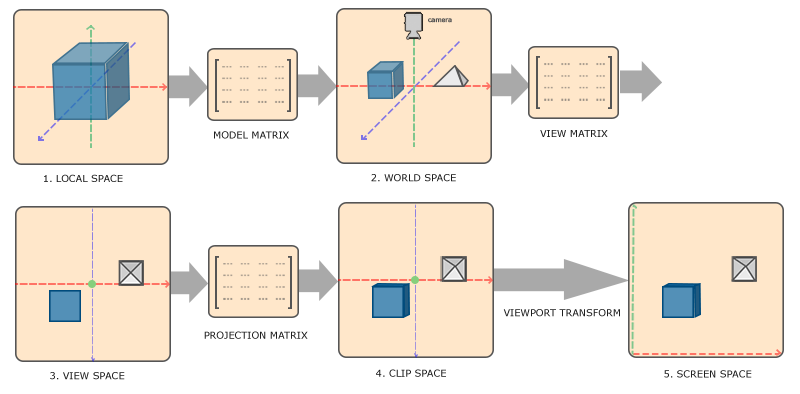
\includegraphics[width=\textwidth]{coordinate-systems.png}
	\caption{Coordinate Systems \cite{fig:view-frustum}}
\end{figure}
\FloatBarrier

We start with the local space, which is the space that we use to define
our objects. Often the objects are centered around the origin of the
local space, but it is up to the modeler to decide where the object is
located. The local space is then transformed into the world space, which
is the 3D space that we use to define the positions of our objects in the scene.
The world space is then transformed into the view space, which is the space that the
camera sees. \cite{fig:view-frustum}

But wait, camera? If you have worked with 3D graphics before, you know
that we need a camera that is used to define the space we can view, aka
the view space. The camera is an object that has a view frustum
with a near and far plane, that is used to define what we can see.

\begin{figure}[hbtp]
	\centering 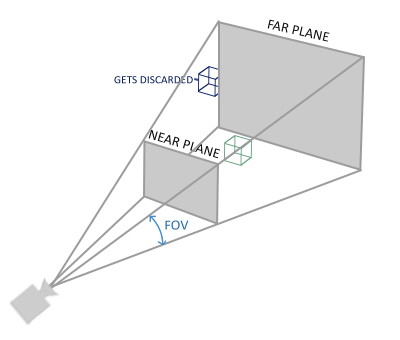
\includegraphics[width=0.60\textwidth]{view-frustum.png}
	\caption{View Frustum \cite{fig:view-frustum}}
\end{figure}
\FloatBarrier

To transform the world space into the view space, we use a view matrix.
Let's briefly talk about matrix transformations and how multiplication
can be used to move, rotate or scale objects in 3D space.

If you have never touched linear algebra before, I suggest you to go over
2Blue1Brown's Essence of Linear Algebra series on YouTube. It is a great
introduction to linear algebra and will help you understand the further topics.

\subsection{Matrix Transformations}

When we have an box in 3D space, we can represent its position as an
array of 3 floats, which are the x, y and z coordinates of its center.
To move the box, we need to add or subtract a value from the x, y or
z coordinate but how can we do that? We can multiply our position with a translation matrix to
move the box. Wait how do we multiply matrices? It's simple. We multiply
the rows of the first matrix with the columns of the second matrix and add them
together. The result is the value of the new matrix at the position where the row and
column intersect.

For example, when we have two matrices A and B, we multiply them like this:

\[
	\begin{bmatrix}
		a & b & c \\
		d & e & f \\
		g & h & i \\
	\end{bmatrix}
	\cdot
	\begin{bmatrix}
		j & k & l \\
		m & n & o \\
		p & q & r \\
	\end{bmatrix}
	=
	\begin{bmatrix}
		(aj + bm + cp) & (ak + bn + cq) & (al + bo + cr) \\
		(dj + em + fp) & (dk + en + fq) & (dl + eo + fr) \\
		(gj + hm + ip) & (gk + hn + iq) & (gl + ho + ir) \\
	\end{bmatrix}
\]

\begin{figure}[hbtp]
	\centering \includesvg[width=0.60\textwidth]{images/matrix-multiplication.svg}
	\caption{Matrix Multiplication \cite{fig:matrix-multiplication}}
\end{figure}
\FloatBarrier

As long as the number of columns in the first matrix is equal to the number
of rows in the second matrix, we can multiply them. The result will have
the same number of rows as the first matrix and the same number of columns
as the second matrix.

When we have a position \{x, y, z\} we cannot just move it by \{tx, ty, tz\}
because multiplying the position with the translation vector would just
multiply the coordinates. But what we need is to add the wanted translation
to the corresponding coordinate.
To do so we need to add a 4th coordinate to the position, which is called
the homogeneous coordinate. This coordinate is usually set to 1 and is used
to set the proportions of the clip space. Don't worry about the clip space
for now, we will talk about it later.

Homogeneous coordinates are used to represent the position of a point with 4
coordinates instead of 3. They have the special property that the homogeneous
coordinates are a multiple of the cartesian coordinates by the w coordinate.

So when we have a point \{1, 2, 3\} in 3D space, we can represent it as
\{1, 2, 3, 1\} in homogeneous coordinates but also as \{2, 4, 6, 2\} or
\{3, 6, 9, 3\} and so on. We will keep the w coordinate at 1, because it is
the easiest to work with.

Our position would then be \{x, y, z, 1\}. Because the w coordinate is the
fourth coordinate, we can multiply the position with a 4x4 matrix where
the forth column is the translation vector. This will add the translation
to the position as long as we keep the diagonal values of the matrix to 1,
so that we don't loose the original position in the calculation.

Therefore we can create the translation that moves the box by \{tx, ty, tz\}
like this:

\[
	\begin{bmatrix}
		1 & 0 & 0 & tx \\
		0 & 1 & 0 & ty \\
		0 & 0 & 1 & tz \\
		0 & 0 & 0 & 1  \\
	\end{bmatrix}
	\cdot
	\begin{bmatrix}
		x \\
		y \\
		z \\
		w \\
	\end{bmatrix}
	=
	\begin{bmatrix}
		x + tx*w \\
		y + ty*w \\
		z + tz*w \\
		w        \\
	\end{bmatrix}
\]

Please note that the w coordinate is changing the x, y and z coordinates,
to adjust the position to our clip space proportions.

But what if we want to rotate the box? We can't just add or
subtract a value from the boxes center to rotate it. We need to tackle each
corner of the box and move it around the center of the box.

To rotate the box, we can multiply the position of each corner with a
rotation matrix.

We can use this knowledge to create a rotation matrix. Lets say we have a line with
the points \{0, 0, 0\} and \{1, 0, 0\}.
When we want to rotate this line around an axis by \(\delta\) degrees, we can apply
the following rotation matrices to the points:

x-axis: \[
	\begin{bmatrix}
		1 & 0            & 0           & 0 \\
		0 & cos(\delta)  & sin(\delta) & 0 \\
		0 & -sin(\delta) & cos(\delta) & 0 \\
		0 & 0            & 0           & 1 \\
	\end{bmatrix}
\]

y-axis: \[
	\begin{bmatrix}
		cos(\delta) & 0 & -sin(\delta) & 0 \\
		0           & 1 & 0            & 0 \\
		sin(\delta) & 0 & cos(\delta)  & 0 \\
		0           & 0 & 0            & 1 \\
	\end{bmatrix}
\]

z-axis: \[
	\begin{bmatrix}
		cos(\delta)  & sin(\delta) & 0 & 0 \\
		-sin(\delta) & cos(\delta) & 0 & 0 \\
		0            & 0           & 1 & 0 \\
		0            & 0           & 0 & 1 \\
	\end{bmatrix}
\]

Let's rotate the line around the y axis:

\[
	P1 =
	\begin{bmatrix}
		cos(\delta) & 0 & -sin(\delta) & 0 \\
		0           & 1 & 0            & 0 \\
		sin(\delta) & 0 & cos(\delta)  & 0 \\
		0           & 0 & 0            & 1 \\
	\end{bmatrix}
	\cdot
	\begin{bmatrix}
		0 \\
		0 \\
		0 \\
		1 \\
	\end{bmatrix}
	=
	\begin{bmatrix}
		0 \\
		0 \\
		0 \\
		1 \\
	\end{bmatrix}
\]

\[
	P2 =
	\begin{bmatrix}
		cos(\delta) & 0 & -sin(\delta) & 0 \\
		0           & 1 & 0            & 0 \\
		sin(\delta) & 0 & cos(\delta)  & 0 \\
		0           & 0 & 0            & 1 \\
	\end{bmatrix}
	\cdot
	\begin{bmatrix}
		1 \\
		0 \\
		0 \\
		1 \\
	\end{bmatrix}
	=
	\begin{bmatrix}
		cos(\delta) \\
		0           \\
		sin(\delta) \\
		1           \\
	\end{bmatrix}
\]

You can see that the origin \(P1\) of the line stays the same, but the end point \(P2\)
of the line has changed. This is because we actually rotate the entire
world space and not the object itself. But because the object is in the
world space, it will also be rotated.

Scaling an object is a bit simpler than rotation. We just multiply
the position of the object with a scaling matrix that
looks like this:

\[
	\begin{bmatrix}
		s_x & 0   & 0   & 0 \\
		0   & s_y & 0   & 0 \\
		0   & 0   & s_z & 0 \\
		0   & 0   & 0   & 1 \\
	\end{bmatrix}
\]

You might see that we simply multiply the x, y and z coordinates with the
scaling factor we want to apply to that axis. So when we want to scale an
object by 2 on the x axis, we would multiply the x coordinate with 2 and
leave the y and z coordinates as they are.

A thing that is important to note is that when applying transformations,
we apply them to the entire world space. This means when rotating, scaling or
moving an object, we are actually rotating, scaling or moving the entire world,
which will also rotate, scale or move the object.

\subsection{View Space}

Now that we know how to transform the world space, we can move the camera
and the objects, so that the camera is the origin of the view space.

To do so we simply take the position of the camera, for example \{1, 2, 3, 1\},
and subtract it from every object in the world space. This will move the
camera to the origin of the view space and keep the objects in the same
position relative to the camera.

\[
	\begin{bmatrix}
		1 & 0 & 0 & -1 \\
		0 & 1 & 0 & -2 \\
		0 & 0 & 1 & -3 \\
		0 & 0 & 0 & 1  \\
	\end{bmatrix}
	\begin{bmatrix}
		x \\
		y \\
		z \\
		w \\
	\end{bmatrix}
	=
	\begin{bmatrix}
		x - 1*w \\
		y - 2*w \\
		z - 3*w \\
		w       \\
	\end{bmatrix}
\]

Now that the camera is the origin of the view space, we need to rotate everything,
so that the camera is looking down the z axis. Lets say we have a camera that
is looking down this direction: \{x,y,z\}. We can create a rotation matrix that
rotates the world space so that the camera is looking down the z axis \{0, 0, z\}.

But first we need to get the angles of the rotation. We can do this by using the
dot product of the camera direction and the z axis. The dot product is simply the
cosine of the angle between two vectors. So when we have two vectors \{x, y, z\}
and \{0, 0, z\}, we can calculate the angle between them by using the dot product.

The dot product looks like this:
\[a \cdot b = |a| * |b| * cos(\theta)\]
\[a \cdot b = a_x * b_x + a_y * b_y + a_z * b_z\]

From here we can divide everything by \(|a| * |b|\) to get \(cos(\theta)= \frac{a \cdot b}{|a| * |b|}\).
Let's calculate the angles we need to rotate the camera to look down the z axis.

We start off by rotating the camera, so that it is looking down the xz plane.
This means that the y coordinate of the camera direction is 0. By taking the dot
product of the camera direction and the x axis on the same hight, we can calculate the angle
we need to rotate the camera around the z axis.

\[
	\begin{bmatrix}
		x \\
		y \\
	\end{bmatrix}
	\cdot
	\begin{bmatrix}
		1 \\
		0 \\
	\end{bmatrix}
	=
	\frac{x}{\sqrt{x^2 + y^2}}
	=
	cos(\theta)
\]

Now we just need to rotate the xz plane around the y axis, so that the camera is looking
up the z axis. We can calculate the angle by taking the dot product of the camera direction
after rotating it around the z axis and the z axis itself

\[
	\begin{bmatrix}
		x \\
		z \\
	\end{bmatrix}
	\cdot
	\begin{bmatrix}
		0 \\
		1 \\
	\end{bmatrix}
	=
	\frac{z}{\sqrt{x^2 + z^2}}
	=
	cos(\theta)
\]

Luckily we don't need to calculate the angles by hand, we can use the
GLM library to calculate the rotation matrix for us. The GLM library is a
header only library that provides us with many useful functions for
mathematical operations.

Don't forget to perform all of this for every object in the world space.
The result will be the view space, where the camera is the origin and
the objects are rotated so that the camera is looking down the z axis.

\subsection{Projection Transformation}

The next step is the transformation from the view space to the clip
space. The clip space is used to define what we can see
on the screen, by clipping everything that is outside of the view frustum.

This task involves transforming the view frustum into an orthographic view
volume, which is a cube with the size of the near plane and the same depth
as the frustum. Then we move the orthographic view volume to the origin
and scale it to the size of the clip space, which is plus and minus the
w coordinate on all axes. The w coordinate is almost always set to 1 by the user,
so the clip space is a cube with the length of 2 on all axes except the z axis,
because the negative z axis is the behind the camera we just have the positive
z axis.

Let's start with the transformation of the view frustum to the orthographic
view volume. We basically need to scale the objects so that the far plane is
the same size as the near plane. Normally the near plane is 0.1 units away and the far
plane is 100 units away but that's up to the user to decide.

When we're looking at the frustum from the side, we can see that the camera and
the far plane create a triangle that can be divided into two right triangles at the
z axis.

\begin{figure}[hbtp]
	\centering \includesvg[width=0.80\textwidth]{images/perspective.svg}
	\caption{View Frustum}
\end{figure} \FloatBarrier

What we need to calculate is yn, which is the new height of the object.
To do so we use the green triangle and the near planes distance on the z axis
(n) to get the following formula:

\[
	\frac{yn}{n} = \frac{y}{z}
\]

We can use this because the triangles sin angle is the same in the green triangle.
When we solve this for yn, we get:

\[
	yn = \frac{y * n}{z}
\]

The same can be applied for the x axis aka the width of the object:

\[
	xn = \frac{x * n}{z}
\]

The z axis stays the same.

So when we have a point \{x, y, z\} in the view space, we need to transform it to \\
\(\{\frac{x * n}{z}, \frac{y * n}{z}, z\}\) to get the orthographic view volume. Unfortunately
there is no way we can divide the x and y value with z with just 3 dimensions.
Here the w coordinate saves us again.

We transfer the z coordinate to the w variable.
This will allow us to divide the x, y and z coordinate by the z coordinate.
So what we want is to transform the point \{x, y, z, w\} to \(\{x * n, y * n, z^2, z\}\).
Keep in mind that the homogeneous coordinate is the same as the 3D coordinate after dividing by w.
This division is called the perspective divide.
So after the perspective divide we get \(\{\frac{x * n}{z}, \frac{y * n}{z}, z\}\) which are
called normalized device coordinates (NDC) or the canonical view volume (CVV).

Okay so what we need is a 4x4 matrix that multiplies the x and y coordinate with n and the z coordinate
with itself. We also need to multiply the w coordinate with z,
to move the z coordinate to the w coordinate. This works because
w is like a scaling factor for the x, y and z coordinate but is often set to 1.

\[
	\begin{bmatrix}
		n & 0 & 0   & 0   \\
		0 & n & 0   & 0   \\
		0 & 0 & m_1 & m_2 \\
		0 & 0 & 1   & 0   \\
	\end{bmatrix}
	\begin{bmatrix}
		x \\
		y \\
		z \\
		w \\
	\end{bmatrix}
	=
	\begin{bmatrix}
		x * n \\
		y * n \\
		z^2   \\
		z     \\
	\end{bmatrix}
\]

Okay we have one last problem. How do we get to \(z^2\) ?
First we have the equation \(z^2 = m_1 * z + m_2\), considering w is 1.
The problem is that there are 2 possible solutions for m1 and m2, which we
can not work with. So we need to add 2 constrains to the equation.
We can just say that we want to apply this equation to the near and far planes z coordinate.
So we will say z = n and z = f. This will give us 2 equations that we can solve for m1 and m2.

\[
	\begin{bmatrix}
		n^2 \\
		f^2 \\
	\end{bmatrix}
	=
	\begin{bmatrix}
		m_1 * n + m_2 \\
		m_1 * f + m_2 \\
	\end{bmatrix}
\]

With this we can now calculate m1 and m2.

\[
	\begin{aligned}
		 & n^2 = m_1 * n + m_2           \\
		 & m_2 = n^2 - m_1 * n           \\
		 & f^2 = m_1 * f + m_2           \\
		 & f^2 = m_1 * f + n^2 - m_1 * n \\
		 & f^2 - n^2 = m_1 * f - m_1 * n \\
		 & f^2 - n^2 = m_1 * (f - n)     \\
		 & m_1 = \frac{f^2 - n^2}{f - n} \\
		 & m_1 = f + n                   \\
		 & m_2 = n^2 - (f + n) * n       \\
		 & m_2 = n^2 - f * n - n^2       \\
		 & m_2 = -f * n
	\end{aligned}
\]

One thing that has to be looked out for is that the near plane and far plane
are not the same because that would result in a division by zero. Also we don't
want the near plane to be 0 because that would result in weird behavior and clipping
into other objects.

Therefor the final matrix looks like this:

\[
	\begin{bmatrix}
		n & 0 & 0     & 0      \\
		0 & n & 0     & 0      \\
		0 & 0 & f + n & -f * n \\
		0 & 0 & 1     & 0      \\
	\end{bmatrix}
\]

This matrix will actually only give us \(z^2\) on the near and far plane. The Objects in between will have
a little offset on the z axis but will remain linearly interpolated between the near and far plane.

Now that we have the orthographic view volume, we need to move it to the origin and
scale it to the size of the CVV. The CVV looks like this from the front:

\begin{figure}[hbtp]
	\centering \includesvg[width=0.60\textwidth]{images/clip-space.svg}
	\caption{Canonical View Volume Front}
\end{figure} \FloatBarrier

It is a coordinate system where the y axis is pointing downwards and the positive of the z axis
is pointing away from us. Each axis ranges from -1 to 1 except the z axis,
which ranges from 0 to 1. This is because the everything negative on the z axis
is behind us and therefor not visible.

Lets first move the orthographic view volumes near planes center to the origin.

\[
	\begin{bmatrix}
		1 & 0 & 0 & -c_x \\
		0 & 1 & 0 & -c_y \\
		0 & 0 & 1 & -c_z \\
		0 & 0 & 0 & 1    \\
	\end{bmatrix}
\]


When the near plane is 0.1 units away, we need to move the orthographic view volume
by 0.1 units on the z axis. So the \(c_z\) value is the distance of the near
plane on the z axis aka n.

For the x and y value we just have to calculate the center of the near plane.
This is done by adding the opposite sides together and then dividing them by 2.
So for \(c_x\) we get \(\frac{l + r}{2}\) and for \(c_y\) we get \(\frac{t + b}{2}\).

Next we scale the orthographic view volume to the size of the CVV.
This is done by multiplying the x, y and z coordinate
with the dimension of the canonical view volume over the size of the orthographic view volume.
We can get the size from subtracting the right side from the left side for the x axis,
the top from the bottom for the y axis and the far from the near plane for the z axis.
So the scaling matrix looks like this:

\[
	\begin{bmatrix}
		\frac{2}{r - l} & 0               & 0               & 0 \\
		0               & \frac{2}{t - b} & 0               & 0 \\
		0               & 0               & \frac{1}{f - n} & 0 \\
		0               & 0               & 0               & 1 \\
	\end{bmatrix}
\]

Now we can combine both transformations to get the final projection matrix:

\[
	\begin{bmatrix}
		1 & 0 & 0 & -\frac{l + r}{2} \\
		0 & 1 & 0 & -\frac{t + b}{2} \\
		0 & 0 & 1 & -n               \\
		0 & 0 & 0 & 1                \\
	\end{bmatrix}
	\cdot
	\begin{bmatrix}
		\frac{2}{r - l} & 0               & 0               & 0 \\
		0               & \frac{2}{t - b} & 0               & 0 \\
		0               & 0               & \frac{1}{f - n} & 0 \\
		0               & 0               & 0               & 1 \\
	\end{bmatrix}
	=
	\begin{bmatrix}
		\frac{2}{r - l} & 0               & 0               & -\frac{l + r}{r - l} \\
		0               & \frac{2}{t - b} & 0               & -\frac{t + b}{b - t} \\
		0               & 0               & \frac{1}{f - n} & -\frac{n}{f - n}     \\
		0               & 0               & 0               & 1                    \\
	\end{bmatrix}
\]

This is the projection matrix that is used to transform the view space to the clip space.
The clip space is then used to determine what is visible on the screen and what is not.
Everything that is visible will now be projected onto the 2D screen.

\subsection{Viewport Transformation}

The viewport is the area on the screen where the image is displayed.
It is defined by the x and y position, the width and height and the
min and max depth and starts at the top left corner of the screen.
The viewport transformation is used to transform the NDC to the screen space.
This is done by scaling the x and y coordinate to the width and height of the viewport,
scaling and moving the z coordinate to the depth range and then adding
half of the width to the x coordinate and subtracting half of the height from the y coordinate
to move the origin to the top left corner of the screen.

\[
	\begin{bmatrix}
		\frac{width}{2} & 0                & 0                   & \frac{width}{2}  \\
		0               & \frac{height}{2} & 0                   & \frac{height}{2} \\
		0               & 0                & maxDepth - minDepth & minDepth         \\
		0               & 0                & 0                   & 1                \\
	\end{bmatrix}
\]

This will transform the NDC to the screen space, but we can also add an x
and y offset to the viewport to move the image around on the screen.
That would mean we need to add the x and y offset when moving
the origin to the top left corner of the screen.

\[
	\begin{bmatrix}
		\frac{width}{2} & 0                & 0                   & \frac{width}{2} + x  \\
		0               & \frac{height}{2} & 0                   & \frac{height}{2} + y \\
		0               & 0                & maxDepth - minDepth & minDepth             \\
		0               & 0                & 0                   & 1                    \\
	\end{bmatrix}
\]

Wow that was a lot of complicated math, but it's important to understand how the world is
projected onto our screen. That's the whole point of 3D graphics after all :P

Don't worry tho if you don't quite understand everything, maybe dive into some other resources to further
understand this topic and until then, do what programmers do best. Copy and paste it from somewhere else.

\section{Stages of the Pipeline}

The Vulkan pipeline consists of multiple stages. Some of them are fixed
and can not be changed, while others are programmable to act as we
want them to. These changeable stages are called shaders and are usually
written in the OpenGL Shading Language (GLSL). Optionally it is possible
to use other shading languages like the High Level Shading Language (HLSL).
These shaders have to be given to the pipeline as compiled SPIR-V bytecode. \cite{spirv}

Lets take a look at the Vulkan pipeline and its stages:

\begin{figure}[hbtp]
	\fontsize{6}{10}\selectfont
	\centering \includesvg[width=1\textwidth]{images/pipeline.svg}
	\caption{Pipeline Structure \cite{fig:pipeline}}
\end{figure} \FloatBarrier

Okay okay, I know that's a lot and there is stuff I haven't talked about
yet, like these Buffers, Images and the Push Constants. Don't worry I
will explain all of these things when going over the stages.

On the left side we have the graphics pipeline and on the right side the
compute pipeline. Now it makes sense that there are different pipelines
for different tasks, right? If we would use the graphics pipeline but
actually just need one shader to edit some data, we would waste a lot
of resources and time sending it though the graphics pipeline.

I'm going to focus on the graphics pipeline and its most important stages.
So some stages will be cut short to better explain the important ones.
In the end you will rarely need to use geometry shaders or tessellation
shaders, but it is important to know that they exist and what they do.

\subsection{Draw}

The draw "stage" is not really a stage, but the command that starts
the rendering process. When we call the vkCmdDraw Command on the GPU,
the pipeline will start processing the data that we have given to
it. \cite{vulkan-spec-draw}

The vkCmdDraw Command is part of the Command Buffer, which is used to
record and execute commands on the GPU. This Command Buffer is then
submitted to a VkQueue, which will execute the commands on the GPU
in the order they were recorded. \cite{command-buffers}


\subsection{Input Assembler}

The input assembler is the first stage of the graphics pipeline. It takes
a vertex and index buffer. \cite{vulkan-spec-pipelines}

Okay we can now finally talk about the input assembler. The input
assembler takes the vertices and indices to create primitives types like
points, lines or triangles. \cite{microsoft-ia}

\newpage

\begin{lstlisting}[language=C++] 

  // Provided by VK_VERSION_1_0 typedef
  enum VkPrimitiveTopology {
    VK_PRIMITIVE_TOPOLOGY_POINT_LIST = 0, VK_PRIMITIVE_TOPOLOGY_LINE_LIST
    = 1, VK_PRIMITIVE_TOPOLOGY_LINE_STRIP =
    2, VK_PRIMITIVE_TOPOLOGY_TRIANGLE_LIST =
    3, VK_PRIMITIVE_TOPOLOGY_TRIANGLE_STRIP =
    4, VK_PRIMITIVE_TOPOLOGY_TRIANGLE_FAN = 5,
    VK_PRIMITIVE_TOPOLOGY_LINE_LIST_WITH_ADJACENCY = 6,
    VK_PRIMITIVE_TOPOLOGY_LINE_STRIP_WITH_ADJACENCY = 7,
    VK_PRIMITIVE_TOPOLOGY_TRIANGLE_LIST_WITH_ADJACENCY = 8,
    VK_PRIMITIVE_TOPOLOGY_TRIANGLE_STRIP_WITH_ADJACENCY = 9,
    VK_PRIMITIVE_TOPOLOGY_PATCH_LIST = 10,
  } VkPrimitiveTopology; 
  \end{lstlisting} \cite{vulkan-spec-primitive-topology}

These are the primitive topology types that the input assembler can
create in Vulkan.  We have to tell the input assembler what type of
topology we want to create, which is usually a triangle strip or list,
but we can also create points or lines.  The difference between a list
and a strip is simple. A list will create a triangle for every 3 indices,
while a strip will create a triangle for every 3 indices and then use
the last 2 vertices of the last triangle to create the next triangle.
The same idea works with lines. The "with adjacency" types are only
used when accessing the geometry stage. We will rarely use
the adjacency types, so don't worry on understanding them now. \cite{vulkan-spec-primitive-topology}

\subsection{Vertex Shader}

The vertex shader is the first programmable stage of the pipeline.
Here we transform the world to our clip space. The vertex shader takes
the vertex data from the input assembler and transforms each vertex
to it's clip space position. \cite{vulkan-tutorial-shader-modules}

But we need to program the transformation ourselves. We can use our new
knowledge of matrices to transform the vertices. To do so we pass the
model, view and projection matrix to the vertex shader via resource descriptors.

When we want to pass data during the rendering process to the shaders,
we have to use resource descriptors. There are multiple types of descriptors, but we will
focus on the uniform buffer descriptor (UBO) which passes data to the shaders
in the form of a buffer.

But first we have to create a descriptor layout that tells the pipeline
what type of data we are passing to which shader. Then we create a descriptor
pool that holds multiple descriptor sets. The descriptor sets are used to
bind the buffers to the shaders and are created from the descriptor pool. \cite{vulkan-tutorial-descriptors}

Descriptors are good to pass constant data to the shaders, but when we
want to pass data that changes frequently we can use push constants.
Push constants are a small amount of data that is stored in the command
buffer. We can assign a minimum of 128 bytes to the push constants, which
is enough to pass 2 4x4 matrices to the shaders. \cite{push-constants}

After that the pipeline performs the perspective divide and returns the
normalized device coordinates.

\subsection{Tessellation}

The tessellation stage is actually divided in 3 stages. The tessellation
control shader, tessellation primitive generator (tessellator) and the tessellation
evaluation shader. Please note that the tessellation stage is optional and will
only be executed if both shaders are defined in the pipeline.\cite{tessellation}

If you are not familiar with tessellation, it is a technique used to
subdivide a polygon, a shape, into smaller polygons without leaving
any gaps in between. This can be used to create more detailed models
without having to pass all the vertex data from the CPU to the GPU. \cite{tessellation}

The tessellation control shader is used to define how many times
our primitive should be subdivided, by defining inner and outer tessellation levels.
It also passes the vertex positions to the evaluation shader. \cite{tessellation}

After setting the tessellation levels, the tessellator subdivides a patch, which is
a new primitive type, into smaller patches.
This can be done in 3 ways: triangles, quads or isolines.
Lets first talk about the tessellation of a triangle.

Vulkan uses barycentric coordinates to subdivide the triangle. Barycentric
coordinates consist, in the case of a triangle, of three variables (u,v,w) that sum up to 1.
Each variable represents the relative position of a vertex in the triangle with 1 being directly
on the vertex. So when we have a triangle with vertices A, B and C, the barycentric coordinates
could be \{0, 0, 1\} for A, \{0, 1, 0\} for B and \{1, 0, 0\} for C, depending on the selected
origin of the triangle. \cite{tessellation}

A point in the triangle ABC, like the center, could be calculated like this:

\[
	\begin{bmatrix}
		1 \\
		1 \\
		1 \\
	\end{bmatrix}
	\div
	3
	=
	\begin{bmatrix}
		\frac{1}{3} \\
		\frac{1}{3} \\
		\frac{1}{3} \\
	\end{bmatrix}
\]

Because the center is equally distant from all vertices,
the barycentric coordinates need to be equal for u, v and w
and when we sum them up they need to equal 1.

First the inner tessellation levels subdivides the patches edges into the desired amount of segments and
creates temporary vertices on the edges of the patch. These vertices are then used to create an
inner triangle by taking the two neighboring vertices of the outer triangles corners and extending perpendicular
lines to the edge of the outer triangle. Where these two lines intersect, a new vertex is created. When you
do this for all three corners it creates the corners of the inner triangle. \cite{tessellation}

\begin{figure}[hbtp]
	\centering 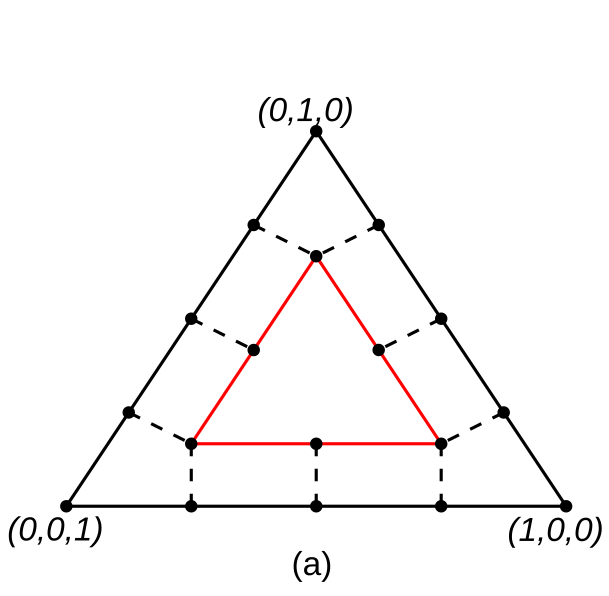
\includegraphics[width=0.4\textwidth]{innertri.png}
	\caption{Inner Tessellation with 4 segments}
	\cite{fig:inner-tessellation}
\end{figure} \FloatBarrier

You can see that the inner tessellation level of four cuts each edge of the outer triangle into four segments.
This is done by calculating the barycentric coordinates of the temporary vertices on the edges. Let's
calculate the barycentric coordinates of the first vertex on the left edge AB.

We need three points where u is always zero because the vertices are on the opposite edge of the corner {1,0,0}
To get the distance of one segment we divide the edge length by the desired segments length.

So the length of one segment is \(\frac{1}{4}\).
For the first vertex we then get \{0, \(\frac{1}{4}\), \(\frac{3}{4}\}\), for the second
vertex \{0, \(\frac{2}{4}\), \(\frac{2}{4}\}\) and for the third vertex \{0, \(\frac{3}{4}\), \(\frac{1}{4}\}\).

We do the same for each edge and then calculate the intersection of the
perpendicular lines to get the inner triangles corner vertices.

For the bottom left corner of the inner triangle we take the
two vertices of the outer triangle \{0, \(\frac{1}{4}\), \(\frac{3}{4}\}\)
and \{\(\frac{1}{4}\), 0, \(\frac{3}{4}\}\).

Now we need to get the direction of the perpendicular line.
This is way easier than it sounds, because our barycentric triangle is equilateral.
That means that when we draw a line to display the height of the triangle and take it's direction,
we get the direction of the perpendicular line to the lower edge.
Luckily, because the triangle stays the same no matter how we rotate it, we can just use
the direction of the height line to get the direction of the
perpendicular lines for each triangle. \cite{equilateral-triangle}

\begin{figure}[htbp]
	\centering 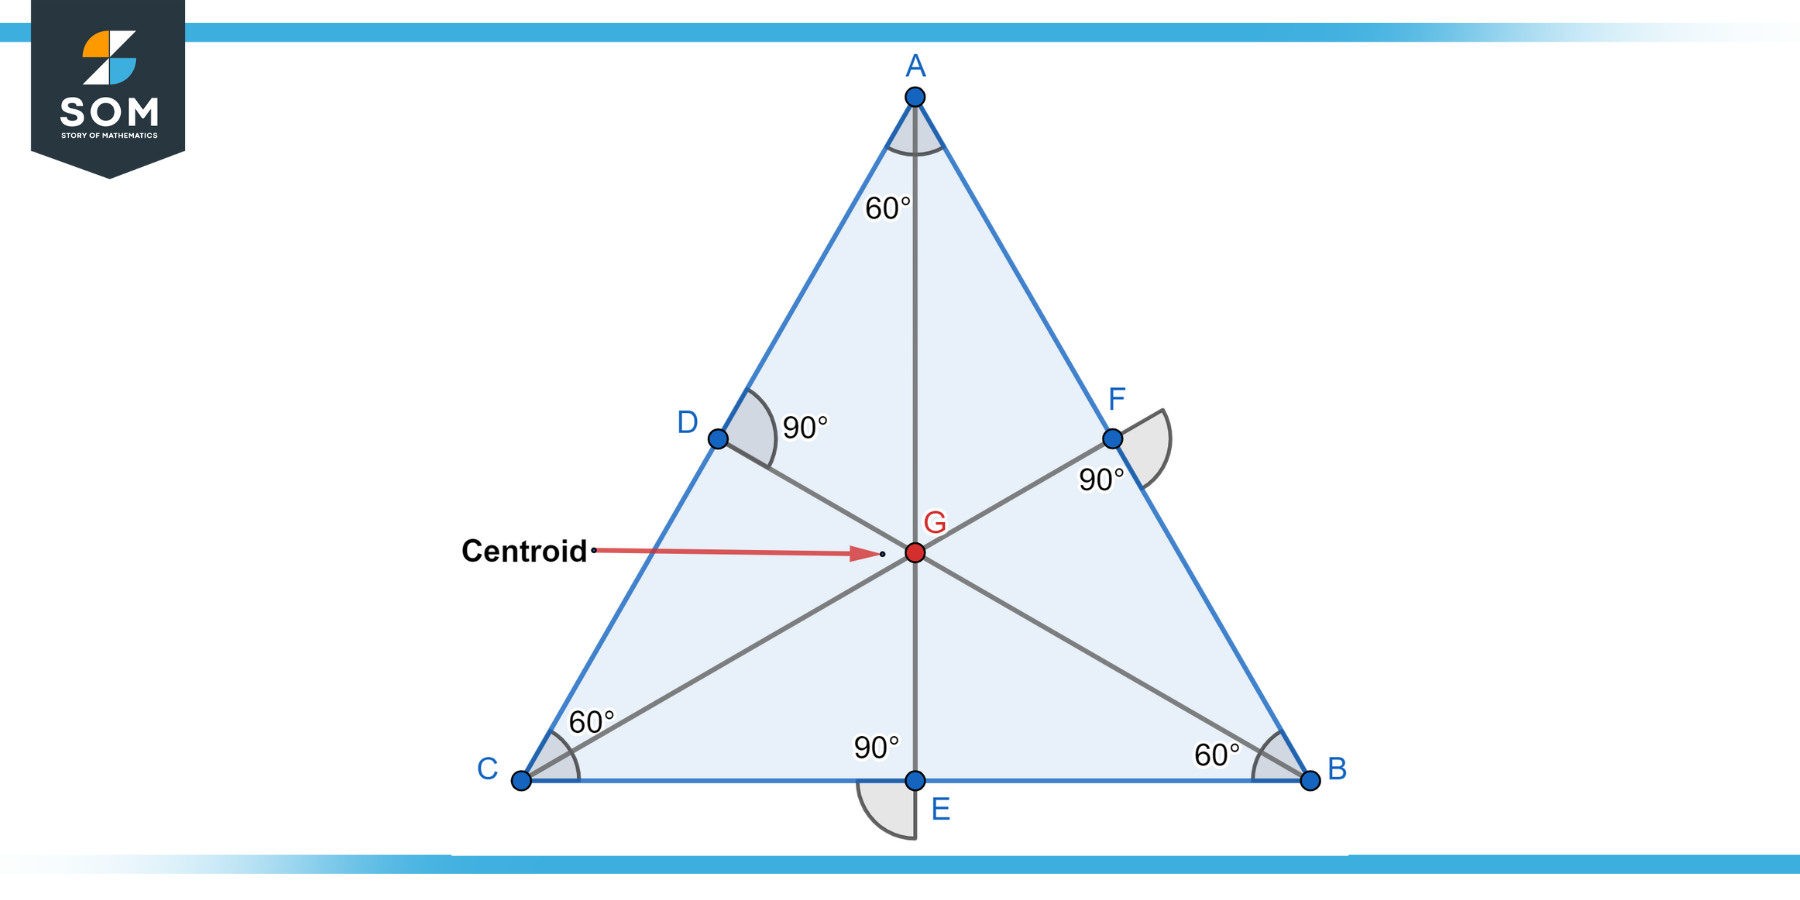
\includegraphics[width=0.7\textwidth]{Equiletral-Triangle.png}
	\caption{Equilateral Triangle}
	\cite{equilateral-triangle}
\end{figure} \FloatBarrier

Considering that we can calculate the direction of the perpendicular line:

\[
	\begin{aligned}
		 & E(\frac{1}{2}, 0, \frac{1}{2})                                                      \\
		 & A(0, 1, 0)                                                                          \\
		 & A - E = (0 - \frac{1}{2}, 1 - 0, 0 - \frac{1}{2}) = (-\frac{1}{2}, 1, -\frac{1}{2}) \\
	\end{aligned}
\]

We can now add this direction to the vertex \(\{\frac{1}{4}, 0, \frac{3}{4}\}\)
to get the perpendicular lines function.

\[
	f(v) = \{\frac{1}{4} - \frac{1}{2}v, 0 + v, \frac{3}{4} - \frac{1}{2}v\}
\]

It's the same for the other points, but we need to change the direction of the perpendicular line.

\[
	f(u) = \{0+u, \frac{1}{4} - \frac{1}{2}u, \frac{3}{4} - \frac{1}{2}u\}
\]

To get the intersection we simply set the functions equal to each other and solve it.

\[
	\begin{aligned}
		     &               & f(v)= f(u)                                                                                \\
		I)   &               & \frac{1}{4} - \frac{1}{2}\cdot v & = u                                                    \\
		II)  &               & v                                & = \frac{1}{4} - \frac{1}{2}\cdot u                     \\
		III) &               & \frac{3}{4} -\frac{1}{2}\cdot v  & = \frac{3}{4} -\frac{1}{2}\cdot u                      \\
		     &               & v                                & = u                                                    \\
		I)   &               & \frac{1}{4} - \frac{1}{2}\cdot u & = u                                                    \\
		     &               & \frac{3}{2}\cdot u               & = \frac{1}{4}                                          \\
		u    & = \frac{1}{6} & v                                & = \frac{1}{6}                      & w & = \frac{4}{6}
	\end{aligned}
\]

Voil\`a, that's how we get the corners of the inner triangle.
Now Vulkan subdivides the inner triangles edges by n-2 with n being the
inner tessellation level. Because our tessellation level is 4
we subdivide the first inner triangles edges into 2 pieces.
The vertex dividing the inner edge is then calculated by projecting a
perpendicular line from the outer edge to the inner edge.
We repeat this until n is smaller than 3, but when we start with n = 2
we will have a tessellation vertex in the center of the triangle. \cite{tessellation}

When we have calculated all inner tessellation vertices we fill the area of the
concentric triangles with triangles by connecting the vertices in a way that
ensures that the triangles are not overlapping. If the inner tessellation level is 2 and
no outer tessellation level is set, the tessellator will connect the corners
of the triangle with the center vertex. \cite{tessellation}
Unfortunately, considering more complicated tessellation, the order in wich the vertices
are created and connected is implementation dependent,
which means that it is up to the GPU to decide how the vertices are connected. \cite{tessellation}

After the inner patches are filled, we discard the outer triangles temporary vertices
and subdivide each edge by it's outer tessellation level.
The tessellator now fills the area of the outer triangle with the outermost inner triangle.
Now that all the triangles are created, the tessellation primitive generator assigns
the vertices their barycentric coordinates (u,v,w)
and passes them to the tessellation evaluation shader. \cite{tessellation}

For Quads and isolines the process is similar, but the patch only has 2 barycentric coordinates.
So we can just calculate the barycentric coordinates as if we were in
an x,y coordinate system. \cite{tessellation}

Quads have 4 outer tessellation levels that subdivide the outer edges
and 2 inner tessellation levels that subdivide the area of the square
into smaller squares. The first inner tessellation level divides the columns
and the second inner tessellation level divides the rows.
At the end the tessellator fills the area of the square with triangles. \cite{tessellation}

Isolines on the other hand is a set of horizontal lines that have a length
of 1 on the u axis and are equally spaced on the v axis.
They only have 2 outer tessellation levels that define how many single lines
are created and in how many segments they are divided.

\begin{figure}[hbtp]
	\centering 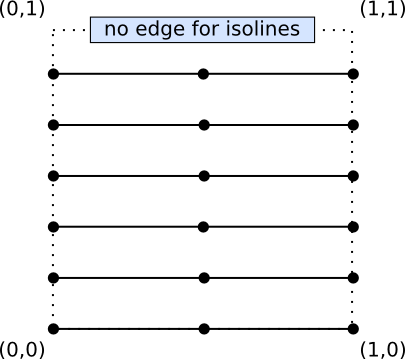
\includegraphics[width=0.4\textwidth]{Tessellation_isoline_6_2.png}
	\caption{Isoline Tessellation (6, 2)}
	\cite{fig:isoline}
\end{figure} \FloatBarrier

These were the possible tessellation types that the tessellator
can work with but there are a few more things to consider for each of them.
For example, we can change the tessellator spacing,
which defines the spacing of the outer tessellation levels.
The tessellator spacing can be either equal, fractional even or fractional odd,
which allow us to have a tessellation level of 2.5 for example. \cite{tessellation}
We can also control the vertex winding order, which defines which side of the triangle
is the front and which is the back. This is important
for culling and lighting calculations. \cite{tessellation}

Please note that all of this is already handled by vulkan
and all we have to do is to set the tessellation levels and optionally spacing
and winding order in the tessellation control shader and pass it over
to the tessellation primitive generator. \cite{tessellation}

After the tessellator created all of the new triangles the tessellation evaluation shader
is called to transform the new vertices to the clip space.
The tessellation evaluation shader takes each barycentric coordinate
and the position of the original triangles corner vertices, that we have forwarded in
the control shader, to calculate the position of the new vertices in clip space. \cite{tessellation}

To do so we can multiply the barycentric coordinates with the corner vertices
and add them together to get the new vertex position.
For a triangle with vertices A, B and C and barycentric coordinates \{u, v, w\}
the new vertex position would be calculated like this:

\[
	\begin{aligned}
		x & = u \cdot A_x + v \cdot B_x + w \cdot C_x \\
		y & = u \cdot A_y + v \cdot B_y + w \cdot C_y \\
		z & = u \cdot A_z + v \cdot B_z + w \cdot C_z \\
	\end{aligned}
\]

After that we can transform them further, adding curvature or displacement to the vertices.
When using a square we can adjust the vertices
by using a 2D texture like a height map to displace the vertices. \cite{tessellation}

One last thing to mention is that when we use a tessellation shader
we actually skip the perspective projection in the vertex shader and
instead do it in the tessellation evaluation shader.
This is because the newly created vertice have to be projected to the clip space
along with the original vertices. \cite{tessellation}

\subsection{Geometry Shader}

The next stage is the geometry shader (GS). The GS is used to create new
primitives and is great at procedural generation of geometry.
That includes creating particles, grass or fur. It takes all the vertices of a primitive
and generates new vertices that are then combined to
either points, line strips or triangle strips.
For example, we could take a single point and create a square around it by emitting 4 new vertices.
These will then be combined to 2 triangles by the pipeline, forming a square. \cite{geometry-shader}

I will not go further into explaining the geometry shader because its
implementation is very dependent on the use case. It is enough to know
some use cases and that we basically can create new primitives with it.

\subsection{Vertex Post Processing}

After all of the previous stages we can do some post processing on the vertices.
This is done by the vertex post processing stage.
Here we have many sub stages that I will go over briefly.

\textbf{Transform Feedback} is used to capture the output of the previous stages
and store it in a feedback buffer. This can be used to
call a new draw command with the stored data. \cite{vertex-post-processing}

\textbf{Viewport Swizzle} is used to change the orientation of the viewport.
For example, we can flip the y axis to display the image upside down.
To achieve this we can define the swizzle for each axis via the VkViewportSwizzleNV struct. \cite{vertex-post-processing}

\textbf{Flat shading} is used to color the whole primitive with one color.
This is done by calculating the color of the first vertex and then
using this color for the whole primitive. \cite{vertex-post-processing}

\textbf{Primitive Clipping} is used to discard primitives that are outside of the clip space.
This is done by checking if the primitive is
completely outside of the clip space and then discarding it. \cite{vertex-post-processing}
When only a part of the primitive is outside of the clip space,
the pipeline will discard that part and create new vertices on the edge of the clip space,
where the primitive would intersects the clip space. \cite{vertex-post-processing}

Clipping is done by checking if the vertex's x, y and z coordinates
are in between -w and w or z\textunderscore min and w for z.
If they are not, the vertex is outside of the clip space and will be discarded.

\textbf{Clipping Shader Outputs} is used to discard the vertex output attributes
that are outside of the clip space.

\textbf{Controlling Viewport W Scaling} can be used to change the w coordinate of the vertex.
This can help to adjust the depth of an object.

\textbf{Coordinate Transformation} is the step where our clip coordinates (x,y,z,w)
are transformed to (x,y,z) by dividing x, y and z by w.
This step is the perspective divide and provides us with
normalized device coordinates (NDC) \cite{vertex-post-processing}

\textbf{Render Pass Transform} can be enabled to rotate the viewport on the xy plane.
This can be used to rotate the image on the screen by either 90, 180 or 270 degrees, using the
VK\textunderscore SURFACE\textunderscore TRANSFORM\textunderscore ROTATE\textunderscore
{degree}\textunderscore BIT\textunderscore KHR attribute. \cite{vertex-post-processing}

\textbf{Controlling the Viewport} is a stage where vulkan scales the NDC
to the dimensions of the viewport. It is also possible to create
scissors to only render a part of the viewport.

\subsection{Rasterization}

This stage of the pipeline converts our primitives into a 2D image.
It takes our viewport and checks which pixels aka fragments are covered by the
primitives and then fills them with the color of the primitive.

Let's take a look on how this is done. Again, there are multiple primitives that can be rasterized:
points, lines and triangles.

We'll start with triangles, because they will be needed for the other types too.

The first step of rasterization is determining if the triangle is front or back facing,
which is done by checking if the area of the triangle is positive or negative.
We can calculate the area of a triangle using the following formula:

\[
	a = -\frac{1}{2} \sum_{i=0}^{n-1} (x_i \cdot y_{i\oplus 1} - x_{i\oplus 1} \cdot y_i)
\]

This probably looks confusing so let me explain it a bit further.
n is the number of vertices in our triangle, which is 3, while i is the current
vertex's index and \(\oplus\) is basically performing \( i+1\) mod n.
So when we have a triangle with vertices A, B and C the sum could look like this:

\[A_x \cdot B_y - B_x \cdot A_y + B_x \cdot C_y - C_x \cdot B_y + C_x \cdot A_y - A_x \cdot C_y\]

or like this:

\[A_x \cdot C_y - C_x \cdot A_y + C_x \cdot B_y - B_x \cdot C_y + B_x \cdot A_y - A_x \cdot B_y\]

depending on the order of the vertices. If your familiar with vector math you might
recognize this as the cross product of two side vectors that originate from the same vertex.
The cross product of these two vectors gives us a vector that is perpendicular to the triangle,
which can either point towards us or away from us.
This is because our 2D display can be seen as a 3D space with the z axis pointing out of the screen.

For example we can take the two vectors \(\vec{AB} = B - A\) and \(\vec{AC} = C - A\)
and calculate the cross product of them to get the normal of the triangle.

To calculate the cross product we can look at this visual representation:

\begin{figure}[hbtp]
	\centering
	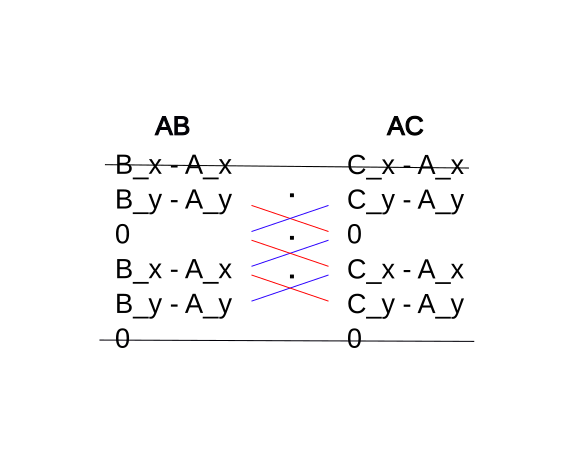
\includegraphics[width=0.5\textwidth]{cross-product.png}
	\caption{Cross Product} \FloatBarrier
\end{figure}

We simply write each vector 2 times under each other, cut out the top and bottom row
and then multiply diagonally, subtract the blue result from the red result
and add each "cross" result together.

In this case we would have:

\[
	\begin{aligned}
		 & (B_y - A_y) \cdot 0 - 0 \cdot (C_x - A_x) = 0                                                                                    \\
		 & 0 \cdot (C_x - A_x) - 0 \cdot (B_x - A_x) = 0                                                                                    \\
		 & (B_x - A_x) \cdot (C_y - A_y) - (C_x - A_x) \cdot (B_y - A_y) =                                                                  \\
		 & B_x \cdot C_y - B_x \cdot A_y - A_x \cdot C_y + A_x \cdot A_y - C_x \cdot B_y + C_x \cdot A_y + A_x \cdot B_y - A_x \cdot A_y  = \\
		 & B_x \cdot C_y - B_x \cdot A_y - A_x \cdot C_y - C_x \cdot B_y + C_x \cdot A_y + A_x \cdot B_y                                    \\
	\end{aligned}
\]

This last therm comes out to our previous formula.
Now that we have a perpendicular vector to the triangle we can calculate the area of the triangle,
because the area of the triangle is half of the cross product.
That's why we multiply the cross product by \(\frac{1}{2}\).
But wait a minute, why is there a minus sign in front of the formula?
This comes from the fact that our z axis is flipped, which means that a positive area
means that the triangle is facing away from us which is not
intuitive. So we flip the sign to get a positive vector.

To actually tell the pipeline what negation is considered front facing
we can set the frontFace attribute in the VkPipelineRasterizationStateCreateInfo
to either \\
VK\textunderscore FRONT\textunderscore FACE\textunderscore CLOCKWISE or
VK\textunderscore FRONT\textunderscore FACE\textunderscore COUNTER\textunderscore CLOCKWISE.
Clockwise means that the triangle is front facing if the area is negative
and counter clockwise then covers the opposite. \cite{rasterization}

Next they are culled according to the cullMode attribute
in the VkPipelineRasterizationStateCreateInfo. This can be set to either
VK\textunderscore CULL\textunderscore MODE\textunderscore NONE, \\
VK\textunderscore CULL\textunderscore MODE\textunderscore FRONT,
VK\textunderscore CULL\textunderscore MODE\textunderscore BACK or \\
VK\textunderscore CULL\textunderscore MODE\textunderscore FRONT\textunderscore AND\textunderscore BACK.
This determines if the front facing, back facing,
both or none of the triangles are discarded. \cite{rasterization}

Next we take the vertices of each triangle and determine its bounding box.
A bounding box is basically the smallest rectangle that
contains the whole triangle. By doing this we don't have to check every fragment
if it is inside the triangle, but only the fragments that are
inside the bounding box. This is done by taking the minimum
and maximum x and y coordinates of the triangle's vertices.

Next we iterate through every fragments center inside the bounding box,
and check if it is inside the triangle.
A point is inside the triangle if it is to the right of all
the triangles edge vectors when it is clockwise oriented
and to the left when it is counter clockwise oriented.
We can check this by calculating the cross product of the edge vectors and the vector
from the first vertex to the fragments position. If the cross product is positive
the point is to the right of the edge, if it is negative it is to the left.
If the cross product is 0 the point is on the edge.

Okay but what if the point is on an edge of adjacent triangles?
How do we know which triangle should be drawn?
For this case graphics APIs usually use the top-left rule.
This rule states that left and top edges are considered to be inside the triangle
while right and bottom edges are considered to be outside. How do we know which edge is which?

A top edge is an edge where the y coordinate is flat and pointing to the right,
so where the y coordinate doesn't change
and the x coordinate is increasing when the winding order is clockwise
or else is decreasing when it is counter clockwise.

A left edge is an edge where the y coordinate is decreasing (clockwise),
which means that it is pointing upwards, because the y axis is flipped.

Is the edge a top or left edge? Then the point is inside the triangle,
otherwise an offset is added to move the point outside of the triangle.

Some of you might not like the idea of checking every fragment inside the bounding box,
because it is very inefficient. There is actually a way to rasterize
a triangle without a bounding box. To do so we have to take a look at
a fact that comes from using the barycentric coordinates.
When we go through the triangle and calculate one of the barycentric coordinates
we can see that the step size we take is always the same
when we go from one fragment in the triangle to the next.
This comes from an intresting property of the barycentric coordinates.
When we go from one fragment to the next the barycentric coordinates
change by a constant amount. This means that we can rasterize a triangle by only checking
the barycentric coordinates of the first fragment and then adding a constant amount
to the barycentric coordinates to get the barycentric coordinates.
If the barycentric coordinates are inside the triangle we draw the pixel, if not we skip it.

We can calculate the constant amount by calculating the barycentric coordinates
of the next pixel and then subtracting the barycentric coordinates
of the current fragment from them. This will give us the constant amount we have to add
to the barycentric coordinates to get the barycentric coordinates of the next fragment.

For lines and points we use the same methods, we just have to draw a box
around the line or point and then check if the fragment is inside this box.
The box drawn is not the bounding box but the thickness of the line or point.

We have two problems left.

First, lines and edges will not look smooth because we only interpolate the color of the vertices.
They will look chunky because we fully color the fragment if the center is inside the box.
To fix this we can use anti-aliasing. Anti-aliasing is a technique used to
smooth the edges of a line or point. We can do this by checking how much of the fragment
is covered by the line and then color the fragment accordingly.

Second, what if we have two triangles that overlap?
We can't just draw the second triangle over the first one.
To fix this we can use a depth buffer. You might have asked yourself why
we need a z coordinate for the vertices. This is because we can use the z coordinate
to determine which fragment is in front of each other. When we rasterize a fragment
we write the z value into an depth buffer and then we check if the z value of the next fragment is
smaller than the z value in the depth buffer. If it is we, draw the fragment and write the new depth
into the depth buffer, if not we skip it.

\subsection{Fragment Shader}

The fragment shader is the last programmable stage of the pipeline.
It takes the fragment data from the rasterization stage and performs
operations on each fragment. This is where we can calculate the color of the fragment.

To do so we need to interpolate the vertex colors.
Fortunately, we already know a way on getting the relative position
of a point to a triangles vertices, the barycentric coordinates.
We can use the barycentric coordinates to interpolate
the color of a vertex to get the color of the pixel.

But how do we get the baricentric coordinates of a pixel?
We can use the same method as before, by calculating the area of the triangle
between to vertices and the pixel. So we take the cross product of one side vector
and the vector from the first vertex to the pixel
and divide it by 2 to get its area. We do this for all 3 sides and then divide them
by the area of the full triangle to get the barycentric coordinates.

For example when we have green vertex A\{1,2\}, red vertex B\{2,3\}
and blue vertex C\{3,2\} and the coordinates of the pixel are
\{2,2.5\} we can calculate the barycentric coordinates like this:

\[
	\begin{aligned}
		\text{Area of the triangle * 2}     & = 2                                             \\
		\text{Area of the triangle ABP * 2} & = \frac{\left| 0.5 - 1 \right|}{2} = 0.25       \\
		\text{Area of the triangle BCP * 2} & = \frac{\left| (-0.5) \right|}{2} = 0.25        \\
		\text{Area of the triangle CAP * 2} & = \frac{\left| (-2) \cdot 0.5 \right|}{2} = 0.5 \\
	\end{aligned}
\]

So the barycentric coordinates are \{0.25, 0.25, 0.5\}.
If you're confused on why I'm using the area times 2, it's because we can safe the
computation of the actual area because we are only caring about
the relative position of the pixel to the vertices, so as long as everything stays
at the same scale it will give us the same answer.

Next we interpolate the colors of the vertices linearly to get the color of the pixel.
This is done by multiplying the color of each vertex, which are floats in the range of 0 to 1,
with the barycentric coordinates and adding them together.

\[
	\begin{aligned}
		r & = 0.25 \cdot A_r + 0.25 \cdot B_r + 0.5 \cdot C_r  \\
		g & = 0.25 \cdot A_g + 0.25 \cdot B_g + 0.5 \cdot C_g  \\
		b & = 0.25 \cdot A_b + 0.25 \cdot B_b + 0.5 \cdot C_b  \\
		\\
		r & = 0.25 \cdot 0 + 0.25 \cdot 1 + 0.5 \cdot 0 = 0.5  \\
		g & = 0.25 \cdot 1 + 0.25 \cdot 0 + 0.5 \cdot 0 = 0.25 \\
		b & = 0.25 \cdot 0 + 0.25 \cdot 0 + 0.5 \cdot 1 = 0.25 \\
	\end{aligned}
\]

Which will give us this color: \{0.5, 0.25, 0.25\}. This will then be converted to the color
space of our surface, which can be sRGB, displayP3 or some other supported color space.
We repeat this for every fragment inside the triangle and then we have our rasterized image.

But we can do more than just interpolate the color of the vertices.
We can also apply lighting, textures and more.

\subsection{Blending}

The last stage of the pipeline is blending. Blending is used to create transparency
and some other graphical effects. There isn't much to say about blending.
It gives us many options to blend the color of the fragment but all of the operations are
performed by the GPU, so we don't have to worry about it.
When blending is complete we have our final framebuffer that we can display.

\section{Drawing Process}

\subsection{Framebuffers}

A framebuffer consists of multiple attachments. An attachment is the buffer
that holds either the color or depth of each fragment.
These buffers are written to by the pipeline and then presented to the screen.
The color attachment is used to store the color of each fragment,
while the depth attachment is used to store the depth of each fragment.
The depth attachment is used to save the z coordinate of each fragment to prevent
drawing over fragments if they are not visible. \cite{framebuffers}

\subsection{Render Pass}

A render pass holds the information about how many color and depth attachments
we have and how they are used in the pipeline.
It can consist of multiple subpasses, which are used to render the scene in multiple steps.
For example, we can render the scene
in one subpass and then apply post processing in another subpass. \cite{render-pass}

\subsection{Swapchain}

The swapchain is used to present the final framebuffer to the screen.
It consists of usually 2 (Double Buffering) or more framebuffers. The best implementation
is to use Triple Buffering, which uses 3 framebuffers.
On a swapchain we can present one framebuffer while we render to another framebuffer.
The presented framebuffer is called the front buffer and the rendered framebuffer
is called the back buffer. Every time a new frame is rendered the
front and back buffers are swapped. This is done to prevent screen tearing.
You know when the screen is cut into 2 different images? That's screen tearing.
It happens when the GPU is rendering to the framebuffer while the screen is reading from it.
But that only happens when we have V-Sync disabled.

There are two problems with Double Buffering. It can cause input lag.
This is because the GPU has to wait for the swapchain to swap the framebuffers
before it can render the next frame. To fix this we can use Triple Buffering.
The other problem occures when the GPU takes longer than one frame.
This will cause the swapchain to wait for the GPU to finish rendering the frame
before it can swap the framebuffers. This will cause the frame
to drop and the game to stutter. To fix this we can use a third buffer
to render to while the GPU is rendering the frame. This way the GPU can
swap the framebuffers without waiting for the GPU to finish rendering the frame. \cite{swapchain}

\section{Conclusion}

This was a brief overview of the Vulkan pipeline and its rendering.
Now that we have a basic understanding of the pipeline we can start
programming our first Vulkan application. In the next chapter we will set up
the Vulkan environment and create a window to render to.

\chapter{Setting up Vulkan}

Because the Setup of Vulkan is highly dependent on your operating system and IDE
I will only give a brief overview of the setup process.

Let's start by setting up our development environment.
First of all we need to to install the Vulkan SDK. You can download it from the
\href{https://vulkan.lunarg.com/sdk/home}{LunarG} website or use your preferred package manager.

Now verify if your GPU and drivers support Vulkan.
To do so go into the Bin folder of the Vulkan SDK and run the
\textit{vkcube.exe} program. If it runs without any errors and display a cube you are good to go.
If not you have to update your drivers or include the Vulkan runtime in your system.

Next we'll need to install GLFW, a library for creating windows and handling input.
We will use it to create a window for our application.
You can download the 64-bit binaries from the \href{https://www.glfw.org/download.html}{GLFW} website or
use your package manager. After downloading the binaries,
extract them to a location that is easy to access.

Because Vulkan does not include a library for
linear algebra operations we will use the \href{https://github.com/g-truc/glm}{OpenGL Mathematics}
(GLM) library. Again, download the library and extract it to a location that is easy to access.

Don't forget to install a C++ and GLSL compiler when needed.

Next you will need to either setup your IDE or write a Makefile to compile your program.

This is a very brief overview of the setup process,
because explaining the setup for every operating system and IDE would be too much.
Please read through this \href{https://vulkan-tutorial.com/Development_environment}{Vulkan Tutorial}
to get a more detailed explanation.

\section{Creating a Window}

Before we can start rendering we need to create an application window,
because vulkan is only a graphics API and doesn't provide a way to create a window.
Do not worry about implementing a window from scratch,
because there are libraries for creating windows for vulkan. We will use the
previously installed open source and multi-platform library GLFW (Graphics Library Framework)
which provides us with a simple API that we can use to create a window and handle input. \cite{glfw}

Let's start by creating a core folder in our source folder. Here all of the core functionalities
of our game engine will be stored. In this folder create a new header file called window.hpp.

Inside we first need to include the GLFW header file and the define of \\
GLFW\textunderscore INCLUDE\textunderscore VULKAN to include the vulkan header files.

\begin{lstlisting}[language=C++]
  #define GLFW_INCLUDE_VULKAN
  #include <GLFW/glfw3.h>
\end{lstlisting}

Next we add a namespace that we want to use for our engine. In my case I will use
the namespace \textit{engine}, but feel free to use the actual name of your engine.
Inside we create our class Window with an constructor that takes the width, height
and name of the window as arguments. We also add a destructor to clean up the window.

\begin{lstlisting}[language=C++]
  #include <string>
  namespace engine {
    class Window {
    public:
      Window(int width, int height, std::string name);
      ~Window();
    };
  }
\end{lstlisting}

The job of the constructor is to initialize a window with the given width, height and name.
So let's create a private helper function that initializes the window. We will call it
\textit{initWindow}. Let's also store the width, height and name of the window in private variables.
After initializing the window we will need a pointer to the window object, so we can access it later.

\begin{lstlisting}[language=C++]
  class Window {
      public:
        Window(int width, int height, std::string name);
        ~Window();
      private:
        void initWindow();
      
        const int width;
        const int height;
      
        std::string name;
        GLFWwindow* window;
    };
\end{lstlisting}


That's the header file for now. Let's implement the defined functions in the source file.
In the Window.cpp file we include the window.hpp file add the namespace and
call the initWindow function in the constructor and set the width, height and name of the class.

\begin{lstlisting}[language=C++]
#include "window.hpp"

namespace engine {
  Window::Window(int width, int height, std::string name)
  : width(width), height(height), name(name) {
      initWindow();
    }
}
\end{lstlisting}

Let's implement the \textit{initWindow} function. First we need to initialize GLFW with the
\textit{glfwInit} function. Then we set two window hints with the \textit{glfwWindowHint} function.
The first hint is the \textit{GLFW\textunderscore CLIENT\textunderscore API} and we set it to
\textit{GLFW\textunderscore NO\textunderscore API}. This tells
GLFW to not create context for the OpenGL API, because it was originaly designed for OpenGL. \cite{client-api-hint}
The second hint is called \textit{GLFW\textunderscore RESIZABLE} and will be set to \textit{GLFW\textunderscore FALSE}
for now, but will be changed later, when implementing a resizable windows.

Once we're done with setting up the window we can create it with the \textit{glfwCreateWindow} function.
It takes the width, height, title as a char pointer, a \textit{GLFWmonitor} pointer, to create a full screen
window and a 5th parameter that is OpenGL specific. Pass in our variables, set the monitor pointer to a
\textit{nullptr}, making our window use windowed mode and do the same for the last parameter.

The output will be a pointer to our created \textit{GLFWwindow} that we can store in our \textit{*window}
variable.

\begin{lstlisting}[language=C++] 
void Window::initWindow() {
  glfwInit();

  glfwWindowHint(GLFW_CLIENT_API, GLFW_NO_API);
  glfwWindowHint(GLFW_RESIZABLE, GLFW_FALSE);

  window = 
    glfwCreateWindow(width, height, name.c_str(), nullptr, nullptr);
}
\end{lstlisting}

Finally we implement our destructor. It will destroy the window with \textit{glfwDestroyWindow()}
and terminate GLFW with \textit{glfwTerminate()}.

\begin{lstlisting}[language=C++]
Window::~Window() {
  glfwDestroyWindow(window);
  glfwTerminate();
}
\end{lstlisting}

Let's test our window by creating a application that creates a window.
Create a app header and source file in the src folder. In the header file we include the window header file,
define a constant \textit{WIDTH} and \textit{HEIGHT} and create a private window object.
We also need a public \textit{run} function that initializes the window and runs the main loop.

\newpage

\begin{lstlisting}[language=C++]
#include "core/window.hpp"

namespace engine {
  class App {
    public:
      static constexpr int WIDTH = 800;
      static constexpr int HEIGHT = 600;

      void run();
    private:
      Window window{WIDTH, HEIGHT, "Vulkan Application"};
  };
}
\end{lstlisting}

In the source file we include the app header file and check in the \textit{run} function if the window
should be closed. While it is not closed we poll the events with \textit{glfwPollEvents()}.

For checking if the window should be closed we create a boolean function \textit{shouldClose} in the
window class and set it to the return value of \textit{glfwWindowShouldClose(window)}.

\begin{lstlisting}[language=C++]
#include "app.hpp"

namespace engine {
  void App::run() {
    while (!window.shouldClose()) {
      glfwPollEvents();
    }
  }
} 
\end{lstlisting}

In the window class add the public \textit{shouldClose} function.
Because it is very simple we can just implement it in the header file.

\begin{lstlisting}[language=C++]
bool shouldClose() { return glfwWindowShouldClose(window); }
\end{lstlisting}

Now we can create a main.cpp that runs the application.
If it fails we return \textit{EXIT\textunderscore FAILURE} and the error.
If it succeeds we return \textit{EXIT\textunderscore SUCCESS}.
We don't need a header file for the main.cpp.

\begin{lstlisting}[language=C++]
#include "app.hpp"
#include <iostream>

int main() {
  engine::App app{};

  try {
    app.run();
  } catch (const std::exception &e) {
    std::cerr << e.what() << '\n';
    return EXIT_FAILURE;
  }

  return EXIT_SUCCESS;
}
\end{lstlisting}

When running our program it should show us a non-resizable window with the title "Vulkan Application".

Great! But we should also remove the windows copy constructor and operator. We don't want to copy the window object,
because we're working with a pointer to the window object. This means that when we copy the window object
we also copy the pointer. When we now delete the original object we also delete the \textit{GLFWwindow}, what
will leave our copy with a dangling pointer. To prevent this potential bug we delete
the copy constructor and copy operator in the window header file.

\begin{lstlisting}
  Window(const Window &) = delete;
  Window &operator=(const Window &) = delete;
\end{lstlisting}

\subsection{Why non-resizable window}

Our current window is not resizable. I've made this decision because when we will
create our SwapChain later it is bound to the windows width an height. So when we
resize or window the SwapChain will not be valid anymore. We will get at it once
we have the base of our engine set up.

\section{Device}

Let's go ahead and setup Vulkan. To do so we have to create an Instance,
a Surface, pick a physical device aka graphics card, create a logical device
and optionally setup validation layers and create a command pool.

What each of these are will be explained further in a second. You might
feel disoriented and confused sometimes when going through this code, but
don't feel discouraged even if you don't understand anything on the first go.
Keep copying the code and come back to this part eventually when you feel more
comfortable with the whole system of Vulkan.

\subsection{Vulkan instance}

The first thing we need to do is to create a Vulkan instance.
A vulkan instance is the connection between our application and the Vulkan library.

Let's start by creating a new header file in the core folder called \textit{device.hpp}
and include the Vulkan header file. In here we will create a constructor, a destructor
a private function to create the Vulkan instance and a private variable to store the instance
and a reference to the window object. We'll also delete the copy and move operators.

\begin{lstlisting}[language=C++]
#include <vulkan/vulkan.h>
#include "window.hpp"

namespace engine {
  class Device {
      public:
        Device(Window &window);
        ~Device();
        
        Device(const Device &) = delete;
        Device &operator=(const Device &) = delete;
        Device(const Device &&) = delete;
        Device &operator=(const Device &&) = delete;

      private:
        void createInstance();
        VkInstance instance;
        Window &window;

        VkSurfaceKHR surface_;
    };
}
\end{lstlisting}

Create the source file and include the header file. In the constructor we call the
\textit{createInstance} function.

\begin{lstlisting}[language=C++]
#include "device.hpp"

namespace engine {
  Device::Device(Window &window) : window{window} {
    createInstance();
  }
}
\end{lstlisting}

To create an instance we need to fill out a struct called \textit{VkInstanceCreateInfo}.
This struct holds information about the application and the Vulkan instance.
The applications information is stored in a struct called \textit{VkApplicationInfo}.
The application info is optional but it is good practice to fill it out. It contains
the name and the version of the application, the engine and the version of the Vulkan API.

\begin{lstlisting}[language=C++]

void Device::createInstance() {
  VkApplicationInfo appInfo = {};
  appInfo.sType = VK_STRUCTURE_TYPE_APPLICATION_INFO;
  appInfo.pApplicationName = "Vulkan Application";
  appInfo.applicationVersion = VK_MAKE_VERSION(1, 0, 0);
  appInfo.pEngineName = "No Engine";
  appInfo.engineVersion = VK_MAKE_VERSION(1, 0, 0);
  appInfo.apiVersion = VK_API_VERSION_1_3;
}
\end{lstlisting}

Please note the \textit{sType} member of the struct. This member is used to tell Vulkan
what type of struct we are using. Why we need this? Vulkan has another member called
\textit{pNext} that is used to extend the struct with additional information. It basically
creates a linked list of structs by pointing to the next struct. The porblem is that there is
no way to know what type of struct is next in the list. The implementation reads the first 4 bytes
of the next struct, which is the \textit{sType} member, to determine the type of the struct and
cast the pointer to the correct struct.

Next we create the \textit{VkInstanceCreateInfo} struct and fill it with the application info.
We also add the extension data from GLFW.
For that we will create a private function called \textit{getRequiredExtensions} that returns
the required extensions as a vector of strings.

\begin{lstlisting}[language=C++]
VkInstanceCreateInfo createInfo = {};
createInfo.sType = VK_STRUCTURE_TYPE_INSTANCE_CREATE_INFO;
createInfo.pApplicationInfo = &appInfo;

std::vector<const char *> extensions = getRequiredExtensions();
createInfo.enabledExtensionCount = static_cast<uint32_t>(extensions.size());
createInfo.ppEnabledExtensionNames = extensions.data();
\end{lstlisting}

The \textit{getRequiredExtensions} function is used to get the required Vulkan extensions
that GLFW needs to create a window with Vulkan. We can get the required extensions with the
\textit{glfwGetRequiredInstanceExtensions} function. To return the extensions as a vector of strings
we need the size of the extensions and a pointer to the extensions as an array. Then we call the function
\textit{glfwGetRequiredInstanceExtensions} which returns the extensions as an array of strings and the size
to the pointer we passed as a parameter to the function. We then copy the extensions to a vector of strings
and return it.

\begin{lstlisting}[language=C++]
std::vector<const char *> getRequiredExtensions() {
  uint32_t glfwExtensionCount = 0;
  const char **glfwExtensions;
  glfwExtensions = glfwGetRequiredInstanceExtensions(&glfwExtensionCount);

  std::vector<const char *> extensions(glfwExtensions, glfwExtensions + glfwExtensionCount);

  return extensions;
}
\end{lstlisting}

Don't forget to add the \textit{getRequiredExtensions} function to the header file.

Finally we create the Vulkan instance with the \textit{vkCreateInstance} function in the
\textit{createInstance} function. We pass the \textit{VkInstanceCreateInfo} struct, a pointer to
a custom allocator, that we will leave as \textit{nullptr} and a pointer to the instance variable.
Custom allocators are used to allocate a range of memory for Vulkan objects. This optimizes memory usage, by
not having to allocate memory for each object separately, but allocating a range of memory and then
sub-allocating the memory for the objects from this range. But we don't need to worry about this for now.

We also have to check if the instance was created successfully. We can do this by checking if the
functions return value is \textit{VK\textunderscore SUCCESS}. If not we throw an exception with an error message.

\begin{lstlisting}[language=C++]
if (vkCreateInstance(&createInfo, nullptr, &instance) != VK_SUCCESS) 
		throw std::runtime_error("Failed to create Vulkan instance");
\end{lstlisting}

Finally we have to clean up the instance in the destructor. We can do this by calling the
\textit{vkDestroyInstance} function with the instance as a parameter.

\begin{lstlisting}[language=C++]
Device::~Device() {
  vkDestroyInstance(instance, nullptr);
}
\end{lstlisting}

Great! Now our instance is created, but there is one more thing I would like to
add to it. Because vulkan is designed to be fast, it doesn't
provide much error checking. To enable error checking we can use validation layers.
Validation layers hook into the function calls of Vulkan and perform additional checks
operation.

\subsection{Validation Layers}

Let's start off by creating a public constant bool enableValidationLayers in the device class header file.
If we want to enable validation layers we set the \textit{NDBUG} macro to 0, otherwise to 1.

\begin{lstlisting}[language=C++]
#ifdef NDEBUG
  const bool enableValidationLayers = false;
#else
  const bool enableValidationLayers = true;
#endif
\end{lstlisting}

Next we add a private vector of strings called \textit{validationLayers} that contains the names of the
validation layers we want to enable.
We will use the \textit{VK\textunderscore LAYER\textunderscore KHRONOS\textunderscore validation}
layer to use the standard error checking provided by Vulkan.

\begin{lstlisting}[language=C++]
const std::vector<const char *> validationLayers = {
  "VK_LAYER_KHRONOS_validation"
};
\end{lstlisting}

Now we have to check if the validation layers, we want to enable, are supported by Vulkan.
To do so we create a private function called \textit{checkValidationLayerSupport} that returns a boolean.
We will use the \textit{vkEnumerateInstanceLayerProperties} function to get the available layers.

First we will create and pass a pointer to a variable that will hold the number of available layers.
Then we will create a vector of \textit{VkLayerProperties} that will hold the available layers.

Then we will iterate thorugh the available layers and check if the the validation layer is in the available layers.
If it is we return true, otherwise we return false.

\begin{lstlisting}[language=C++]
bool Device::checkValidationLayerSupport() {
  uint32_t layerCount;
  vkEnumerateInstanceLayerProperties(&layerCount, nullptr);

  std::vector<VkLayerProperties> availableLayers(layerCount);
  vkEnumerateInstanceLayerProperties(&layerCount, availableLayers.data());

  for (const char *layerName : validationLayers) {
      bool layerFound = false;

      for (const auto layerProperty : availableLayers) {
          if (strcmp(layerName, layerProperty.layerName) == 0) {
              layerFound = true;
              break;
            }
        }

      if (!layerFound)
      return false;
    }
  return true;
}
\end{lstlisting}

At the top of the \textit{createInstance} function we will check if the validation layers are supported
when the \textit{enableValidationLayers} constant is set to true. If the validation layers are not
supported we throw an exception with an error message.

\newpage

\begin{lstlisting}[language=C++]
if (enableValidationLayers && !checkValidationLayerSupport())
  throw std::runtime_error("Requested validation layers are not supported!");
\end{lstlisting}

GLFW needs another extension to make the validation layers works. This extension is called
\textit{VK\textunderscore EXT\textunderscore DEBUG\textunderscore UTILS\textunderscore EXTENSION\textunderscore NAME}.
So let's add this extension to the \textit{getRequiredExtensions} function.

\begin{lstlisting}[language=C++]
std::vector<const char *> getRequiredExtensions() {
  uint32_t glfwExtensionCount = 0;
  const char **glfwExtensions;
  glfwExtensions = glfwGetRequiredInstanceExtensions(&glfwExtensionCount);

  std::vector<const char *> extensions(glfwExtensions, glfwExtensions + glfwExtensionCount);

  if (enableValidationLayers)
    extensions.push_back(VK_EXT_DEBUG_UTILS_EXTENSION_NAME);

  return extensions;
}
\end{lstlisting}

To activate the validation layers we have to add them to the \textit{VkInstanceCreateInfo} struct.
We also have to add a debug messenger to get the validation layer messages. To do so we can
use the \textit{VkDebugUtilsMessengerCreateInfoEXT} struct that we will use to extend the
\textit{VkInstanceCreateInfo} struct. Let's add a private function called \textit{populateDebugMessenger}
that takes a \textit{VkDebugUtilsMessengerCreateInfoEXT} struct reference as an argument fills it with
the desired values. Then we add the debug messenger to the \textit{VkInstanceCreateInfo} struct.

\newpage

\begin{lstlisting}[language=C++]
if (enableValidationLayers) {
createInfo.enabledLayerCount = static_cast<uint32_t>(validationLayers.size());
createInfo.ppEnabledLayerNames = validationLayers.data();

VkDebugUtilsMessengerCreateInfoEXT debugCreateInfo;
populateDebugMessenger(debugCreateInfo);

createInfo.pNext = (VkDebugUtilsMessengerCreateInfoEXT *) &debugCreateInfo;

} else {
createInfo.enabledLayerCount = 0;
createInfo.pNext = nullptr;
}
\end{lstlisting}

\begin{lstlisting}[language=C++]
void Device::populateDebugMessenger(VkDebugUtilsMessengerCreateInfoEXT &createInfo) {
  createInfo = {};
  createInfo.sType = VK_STRUCTURE_TYPE_DEBUG_UTILS_MESSENGER_CREATE_INFO_EXT;
  createInfo.messageSeverity = VK_DEBUG_UTILS_MESSAGE_SEVERITY_WARNING_BIT_EXT |
                                    VK_DEBUG_UTILS_MESSAGE_SEVERITY_ERROR_BIT_EXT;
  createInfo.messageType = VK_DEBUG_UTILS_MESSAGE_TYPE_GENERAL_BIT_EXT | 
                                VK_DEBUG_UTILS_MESSAGE_TYPE_VALIDATION_BIT_EXT |
                                VK_DEBUG_UTILS_MESSAGE_TYPE_PERFORMANCE_BIT_EXT;
  createInfo.pfnUserCallback = debugCallback;
  createInfo.pUserData = nullptr;
}
\end{lstlisting}

The \textit{messageSeverity} member of the \textit{VkDebugUtilsMessengerCreateInfoEXT} struct
is used to determine which message severity levels should be used. We basically have 4 levels of
severity. Verbose, Info, Warning and Error. Each of them is assigned a bit. For example the
\textit{VK\textunderscore DEBUG\textunderscore UTILS\textunderscore MESSAGE\textunderscore SEVERITY\textunderscore WARNING\textunderscore BIT\textunderscore EXT}
is equal to 0x00000100 and the \\
\textit{VK\textunderscore DEBUG\textunderscore UTILS\textunderscore MESSAGE\textunderscore SEVERITY\textunderscore ERROR\textunderscore BIT\textunderscore EXT}
is equal to 0x00001000. We can combine these bits with the bitwise OR operator to get the desired severity level
0x00001100. When we get a message it has a severity level assigned to it. This level is then AND combinded to the
\textit{messageSeverity} member. The same is done with the \textit{messageType} member.

If the results are not 0 the \textit{pfnUserCallback} function is called that
outputs the message.  If you want to pass user data to the callback function you can do so with the
\textit{pUserData} member.

Let's implement the \textit{debugCallback} function.
It takes the severity, type, pCallbackData and pUserData as arguments and returns a \textit{VkBool32}
which has to be \textit{VK\textunderscore FALSE}.

\begin{lstlisting}[language=C++]
static VKAPI_ATTR VkBool32 VKAPI_CALL debugCallback(
VkDebugUtilsMessageSeverityFlagBitsEXT messageSeverity,
VkDebugUtilsMessageTypeFlagsEXT messageType,
const VkDebugUtilsMessengerCallbackDataEXT *pCallbackData,
void *pUserData) {
		std::cerr << "Debug callback" << pCallbackData->pMessage << std::endl;
		return VK_FALSE;
	}
\end{lstlisting}

The \textit{VKAPI\textunderscore ATTR} and \textit{VKAPI\textunderscore CALL} are enables Vulkan to
use the correct calling convention for the function. For now we will just output the message to the
console but you can do whatever you want with the message.

Next we have to create the debug messenger with the \textit{vkCreateDebugUtilsMessengerEXT} function.
But before we can do that we have to load the function with the \textit{vkGetInstanceProcAddr} function.
We'll start off by adding a function in the constructor that setups the debug messenger and then
use a generic function to load the function and create the messenger. Let's also add a private
variable that stores the debug messenger.

\newpage

\begin{lstlisting}[language=C++]
//device.hpp
void setupDebugMessenger();
VkDebugUtilsMessengerEXT debugMessenger;
\end{lstlisting}

\begin{lstlisting}[language=C++]
//device.cpp
Device::Device(Window &window) : window{window} {
  createInstance();
  setupDebugMessenger();
}

void Device::setupDebugMessenger() {
  if (!enableValidationLayers) return;

  VkDebugUtilsMessengerCreateInfoEXT createInfo;
  populateDebugMessenger(createInfo);

  if (CreateDebugUtilsMessengerEXT(instance, &createInfo, nullptr, &debugMessenger) != VK_SUCCESS)
    throw std::runtime_error("Failed to set up debug messenger");
}

VkResult CreateDebugUtilsMessengerEXT(
  VkInstance instance, const VkDebugUtilsMessengerCreateInfoEXT *pCreateInfo,
  VkAllocationCallbacks *pAllocator, VkDebugUtilsMessengerEXT *pDebugMessenger) {
    auto func = (PFN_vkCreateDebugUtilsMessengerEXT) vkGetInstanceProcAddr(instance, "vkCreateDebugUtilsMessengerEXT");
    if (func != nullptr) 
      return func(instance, pCreateInfo, pAllocator, pDebugMessenger);
    else return VK_ERROR_EXTENSION_NOT_PRESENT;
\end{lstlisting}

The \textit{CreateDebugUtilsMessengerEXT} function trys to load the \textit{vkCreateDebugUtilsMessengerEXT}
function with the \textit{vkGetInstanceProcAddr} function. If the function is loaded successfully
we create the debug messenger with that function and return the result. If the function is not loaded
we return \textit{VK\textunderscore ERROR\textunderscore EXTENSION\textunderscore NOT\textunderscore PRESENT}.

And don't forget to destroy the debug messenger in the destructor if the validation layers are enabled.
To do so we'll have to load the \textit{vkDestroyDebugUtilsMessengerEXT} function with the same
function we used to load the \textit{vkCreateDebugUtilsMessengerEXT} function. Let's add a lokal helper function
to the device class that destroys the debug messenger called \textit{destroyDebugUtilsMessengerEXT}.

\begin{lstlisting}[language=C++]
//device.cpp
Device::~Device() {
  if (enableValidationLayers)
    destroyDebugUtilsMessengerEXT(instance, debugMessenger, nullptr);

  vkDestroyInstance(instance, nullptr);
}

void destroyDebugUtilsMessengerEXT(VkInstance instance, 
  VkDebugUtilsMessengerEXT debugMessenger, 
  const VkAllocationCallbacks *pAllocator) {
    auto func = (PFN_vkDestroyDebugUtilsMessengerEXT) vkGetInstanceProcAddr(instance, "vkDestroyDebugUtilsMessengerEXT");
    if (func != nullptr) 
      func(instance, debugMessenger, pAllocator);
  }
\end{lstlisting}

\subsection{Surface}

Now that we have some error checking and a window, we need a surface to render on.
GLFW provides us with a function to create a surface. Let's add a private function,
in the window class, called
\textit{createWindowSurface} that creates a surface with the \textit{glfwCreateWindowSurface} function.
It takes the instance and a pointer to the surface as arguments. So add a private variable
to store the surface and a \textit{createSurface} function in the device class.

\begin{lstlisting}[language=C++]
//device.cpp
Device::Device(Window &window) : window{window} {
		createInstance();
		setupDebugMessenger();
		createSurface();
	}

void Device::createSurface() {
	window.createWindowSurface(instance, &surface);
}
\end{lstlisting}

\begin{lstlisting}[language=C++]
//window.cpp
void Window::createWindowSurface(VkInstance instance, VkSurfaceKHR *surface) {
	if (glfwCreateWindowSurface(instance, window, nullptr, surface) != VK_SUCCESS)
		throw std::runtime_error("Surface creation failed!");
}
\end{lstlisting}

We also have to destroy the surface in the destructor of the device class.

\begin{lstlisting}[language=C++]
Device::~Device() {
  if (enableValidationLayers)
    destroyDebugUtilsMessengerEXT(instance, debugMessenger, nullptr);

  vkDestroySurfaceKHR(instance, surface, nullptr);
  vkDestroyInstance(instance, nullptr);
}
\end{lstlisting}

\subsection{Physical Device}

The physical device is the actual graphics card that we will use to render our scene. We
can use either one or multiple physical devices to render our scene. But for now we will
only use one.

The first thing we need to do is to get the available physical devices. Then we check each of them
until we find a suitable device.

Let's begin with defining our helper functions \textit{pickPhysicalDevice} and \textit{isDeviceSuitable}
and a private variable to store the physical device.

\begin{lstlisting}[language=C++]
//device.hpp
private:
...
VkPhysicalDevice physicalDevice = VK_NULL_HANDLE;
VkPhysicalDeviceProperties properties;
void pickPhysicalDevice();
bool isDeviceSuitable(VkPhysicalDevice device);
\end{lstlisting}

Next we call the \textit{pickPhysicalDevice} function in our constructor. Inside the function we
first need to get all available physical devices with the \textit{vkEnumeratePhysicalDevices} function.
Then we iterate through the devices and check until we find a suitable device with the \textit{isDeviceSuitable}
function. In case the loop ends without finding a suitable device we check if the physical device is
\textit{VK\textunderscore NULL\textunderscore HANDLE}. If it is we throw an exception with an error message.
Finally we get the properties of our device with \textit{vkGetPhysicalDeviceProperties} and store it in a private variable.

\begin{lstlisting}[language=C++]
//device.cpp
Device::Device(Window &window) : window{window} {
  ...
  pickPhysicalDevice();
}

void Device::pickPhysicalDevice(){
  uint32_t deviceCount = 0;
  vkEnumeratePhysicalDevices(instance, &deviceCount, nullptr);

  if(deviceCount == 0)
    throw std::runtime_error("Failed to find a GPU that supports Vulkan!");

  std::vector<VkPhysicalDevice> devices(deviceCount);
  vkEnumeratePhysicalDevices(instance, &deviceCount, &devices);

  for(const auto &device : devices){
    if(isDeviceSuitable(device)){
      physicalDevice = device;
      break;
    }
  }

  if(physicalDevice == VK_NULL_HANDLE)
    throw std::runtime_error("No Device was suitable!");

  vkGetPhysicalDeviceProperties(physicalDevice, &properties);
  \\optional
  std::cout << "Physical Device: " << properties.deviceName << std::endl;
}
\end{lstlisting}

The \textit{isDeviceSuitable} function is used to check if the device is suitable for our application.
In here we will check if the device can process graphics, present images on the surface, supports the required extensions
and if it is swapchain adequate.

Okay, let's start by checking if the device supports graphics commands. This data is stored in
the \textit{VkQueueFamilyProperties} struct and needs to be queried with the \textit{vkGetPhysicalDeviceQueueFamilyProperties}
function from the physical device.

Before I explain further I have to explain what a queue and a queue family is. Do you remember
when I mentioned Command Buffers? These are used to send commands to the GPU. For example, to run a
graphics pipeline we would add the \textit{vkCmdDraw} command to the command buffer. This command
buffer then has to be submitted to a queue. A queue determines the order in which the command buffers
are executed.

But here is the catch. Not all queues can execute all command buffers. One queue might be able to
execute graphics commands, while another queue might be able to execute compute commands and so on.
Therefore we have to check if the device supports the required queues, which are graphics for now.

We can get the available queues with the \textit{vkGetPhysicalDeviceQueueFamilyProperties} function.
It returns all queues with the same capabilities as a queue family. So when the GPU has 2 queues
that can execute graphics commands we get a queue family with a queue count of 2 and a flag that
indicates that it can execute graphics commands.

Let's go ahead and add a private function called \textit{findQueueFamilies} that returns a struct
that contains the indices of the graphics and present queue family. We will call this struct
\textit{QueueFamilyIndices} and it will contain an optional uint32\_t for the graphics queue family,
an optional uint32\_t for the present queue family and a function \textit{isComplete} that returns
true if the graphics and present queue family are set.

Inside \textit{findQueueFamilies} we can check if the queue family can execute graphics commands by iterating through each queue family
and checking if its \textit{queueFlags} member has the \textit{VK\textunderscore QUEUE\textunderscore GRAPHICS\textunderscore BIT} set.
If it is we set the graphics queue family index to the current index. We also check for a queue family that can present images
on a given surface with the \textit{vkGetPhysicalDeviceSurfaceSupportKHR} function. If it does we set the present queue family index
to the current index.

We will then return the \textit{QueueFamilyIndices} struct from the \textit{findQueueFamilies} function. We will need the indices
to create the device.

\begin{lstlisting}[language=C++]
\\device.hpp

struct QueueFamilyIndices {
  std::optional<uint32_t> graphicsFamily;
  std::optional<uint32_t> presentFamily;

  bool isComplete() {
    return graphicsFamily.has_value() && presentFamily.has_value();
  }
};
\end{lstlisting}

\begin{lstlisting}[language=C++]
\\device.cpp

bool Device::isDeviceSuitable(VkPhysicalDevice device) {
  QueueFamilyIndices indices = findQueueFamilies(device);

  return indices.isComplete();
}

QueueFamilyIndices Device::findQueueFamilies(VkPhysicalDevice device) {
  QueueFamilyIndices indices;

  uint32_t queueFamilyCount = 0;
  vkGetPhysicalDeviceQueueFamilyProperties(device, &queueFamilyCount, nullptr);

  std::vector<VkQueueFamilyProperties> queueFamilies(queueFamilyCount);
  vkGetPhysicalDeviceQueueFamilyProperties(device, &queueFamilyCount, queueFamilies.data());

  int i = 0;
  for (const auto &queueFamily : queueFamilies) {
    if (queueFamily.queueCount > 0 && queueFamily.queueFlags & VK_QUEUE_GRAPHICS_BIT)
      indices.graphicsFamily = i;

    VkBool32 presentSupport = false;
    vkGetPhysicalDeviceSurfaceSupportKHR(device, i, surface, &presentSupport);

    if (queueFamily.queueCount > 0 && presentSupport)
      indices.presentFamily = i;

    if (indices.isComplete())
      break;

    i++;
  }

  return indices;
}
\end{lstlisting}

Now we check if the device supports the required extensions. For that we will create another helper function
called \textit{checkDeviceExtensionSupport} that returns a boolean. We will use the \textit{vkEnumerateDeviceExtensionProperties}
to get the available extensions. Then we will create a set of strings that contains the required extensions which will be the
\textit{VK\textunderscore KHR\textunderscore SWAPCHAIN\textunderscore EXTENSION\textunderscore NAME} for now. We will then iterate through
the available extensions and remove the required extensions from the set. If the set is empty we return true, otherwise false.

\begin{lstlisting}[language=C++]
//device.hpp

private:
  bool checkDeviceExtensionSupport(VkPhysicalDevice device);
  const std::vector<const char *> deviceExtensions = {
    VK_KHR_SWAPCHAIN_EXTENSION_NAME
  };
\end{lstlisting}

\begin{lstlisting}[language=C++]
//device.cpp
bool Device::isDeviceSuitable(VkPhysicalDevice device) {
  QueueFamilyIndices indices = findQueueFamilies(device);
  bool extensionsSupported = checkDeviceExtensionSupport(device);

	return indices.isComplete() && extensionsSupported;
}

bool Device::checkDeviceExtensionSupport(VkPhysicalDevice device) {
  uint32_t extensionCount;
  vkEnumerateDeviceExtensionProperties(device, nullptr, &extensionCount, nullptr);

  std::vector<VkExtensionProperties> availableExtensions(extensionCount);
  vkEnumerateDeviceExtensionProperties(device, nullptr, &extensionCount, availableExtensions.data());

  std::set<std::string> requiredExtensions(deviceExtensions.begin(), deviceExtensions.end());

  for (const auto &extension : availableExtensions)
    requiredExtensions.erase(extension.extensionName);

  return requiredExtensions.empty();
}
\end{lstlisting}

Another thing we have to check is if the device is adequate for a swapchain and simultaneously
get some required data for creating the swapchain.

Each device has a set of capabilities, like the minimum and maximum images for a swapchain
and the minimum and maximum width and height of the image, that we can get with the
\textit{vkGetPhysicalDeviceSurfaceCapabilitiesKHR} function.

We also need the formats and the present modes that the device supports via the
\textit{vkGetPhysicalDeviceSurfaceFormatsKHR} and the \textit{vkGetPhysicalDeviceSurfacePresentModesKHR}
functions.

Let's go ahead and create another struct called \textit{SwapChainSupportDetails} that stores the capabilities,
formats and present modes.

\begin{lstlisting}[language=C++]
//device.hpp

struct SwapChainSupportDetails{
  VkSurfaceCapabilitiesKHR capabilities;
  std::vector<VkSurfaceFormatKHR> formats;
  std::vector<VkPresentModeKHR> presentModes;
}
\end{lstlisting}

Next we create a function called \textit{querySwapChainSupport} that returns our
\textit{SwapChainSupportDetails} struct with the data.

\begin{lstlisting}[language=C++]
//device.cpp

bool Device::isDeviceSuitable(VkPhysicalDevice device){
  ...
  bool swapChainAdequate = false;
  if(extensionsSupported){
    SwapChainSupportDetails swapChainSupport = querySwapChainSupport(device);
    swapChainAdequate = !swapChainSupport.formats.empty() &&
                        !swapChainSupport.presentModes.empty();
  }

  return indices.isComplete() && extensionsSupported && swapChainAdequate;
}

SwapChainSupportDetails Device::querySwapChainSupport(VkPhysicalDevice device){
  SwapChainSupportDetails details;
  vkGetPhysicalDeviceSurfaceCapabilitiesKHR(device, surface_, &details.capabilities);

  uint32_t formatCount;
  vkGetPhysicalDeviceSurfaceFormatsKHR(device, surface_, &formatCount, nullptr);

  if(formatCount != 0){
    details.formats.resize(formatCount);
    vkGetPhysicalDeviceSurfaceFormatsKHR(device, surface_, &formatCount, details.formats.data());
  }

  uint32_t presentModeCount;
  vkGetPhysicalDeviceSurfacePresentModesKHR(device, surface_, &presentModeCount, nullptr);

  if(presentModeCount != 0){
    details.presentModes.resize(presentModeCount);
    vkGetPhysicalDeviceSurfacePresentModesKHR(device, surface_, &presentModeCount, details.presentModes.data());
  }

  return details;
}
\end{lstlisting}

Finally we check if the device supports anisotropic filtering. Anisotropic filtering is a technique
that enhances the image quality of textures on surfaces, by reducing blurriness that can occur when
rendering texture on a sharp angle. We'll look deeper into this topic later.

We can check if the device supports anisotropic filtering by checking the \textit{VkPhysicalDeviceFeatures}
struct that contains the features of the device. \textit{vkGetPhysicalDeviceFeatures} returns the features
of the device, which contains the boolean \textit{samplerAnisotropy} member.

\begin{lstlisting}[language=C++]
bool Device::isDeviceSuitable(VkPhysicalDevice device){
  ...
  VkPhysicalDeviceFeatures supportedFeatures;
  vkGetPhysicalDeviceFeatures(device, &supportedFeatures);

  return indices.isComplete() && extensionsSupported && swapChainAdequate && supportedFeatures.samplerAnisotropy;
}
\end{lstlisting}

That's it we have now picked a physical device that is suitable for our application. But please note that
we just take the first suitable device we find, which is not the best practice. You should rather
rate the devices by certain factors. For example, you could favor a dedicated GPU over an integrated GPU.

For now we will just take the first suitable device we find.

\subsection{Logical Device}

We currently have a physical device but no interface to interact with it. This interface is provided
by a logical device that we will create in the next step. Let's add a private function called
\textit{createLogicalDevice} that creates the logical device and a private variable to store the device.
We'll also create our queues here and will need a \textit{VkQueue} variable for each queue;

\begin{lstlisting}[language=C++]
//device.hpp
private:
  ...
  VkDevice device_;
  VkQueue graphicsQueue_;
  VkQueue presentQueue_;
  void createLogicalDevice();
\end{lstlisting}

The logical device is created with the \textit{vkCreateDevice} function. We have to specify the
queues that we want to create for the device. We do so by populating the \textit{VkDeviceQueueCreateInfo}
struct and add it to the \textit{VkDeviceCreateInfo} struct. We'll need to specify the queue family index,
the amount of queues and the priority of the queues. We'll keep the same priority for all queues for now,
but you can adjust the priority to your needs. We also have to specify the device features in an
\textit{VkPhysicalDeviceFeatures} struct, that we want to enable, which will be sampler anisotropy for now.
We also have to specify the extensions that we want to enable,
which is the swapchain extension in our \textit{deviceExtensions} vector.

When we create the logical device we also have to check if the creation was successful. If not we throw
an exception with an error message. After that we retrieve the queues from the device with the
\textit{vkGetDeviceQueue} function.

\begin{lstlisting}[language=C++]
//device.cpp
Device::Device(Window &window) : window{window} {
  ...
  createLogicalDevice();
}

void Device::createLogicalDevice(){
  QueueFamilyIndices indices = findQueueFamilies(physicalDevice);

  std::vector<VkDeviceQueueCreateInfo> queueCreateInfos;
  std::set<uint32_t> uniqueQueueFamilies = {indices.graphicsFamily.value(), indices.presentFamily.value()};

  float queuePriority = 1.0f;
  for(uint32_t queueFamily : uniqueQueueFamilies){
    VkDeviceQueueCreateInfo queueCreateInfo = {};
    queueCreateInfo.sType = VK_STRUCTURE_TYPE_DEVICE_QUEUE_CREATE_INFO;
    queueCreateInfo.queueFamilyIndex = queueFamily;
    queueCreateInfo.queueCount = 1;
    queueCreateInfo.pQueuePriorities = &queuePriority;
    queueCreateInfos.push_back(queueCreateInfo);
  }

  VkPhysicalDeviceFeatures deviceFeatures = {};
  deviceFeatures.samplerAnisotropy = VK_TRUE;

  VkDeviceCreateInfo createInfo = {};
  createInfo.sType = VK_STRUCTURE_TYPE_DEVICE_CREATE_INFO;
  createInfo.queueCreateInfoCount = static_cast<uint32_t>(queueCreateInfos.size());
  createInfo.pQueueCreateInfos = queueCreateInfos.data();
  createInfo.enabledExtensionCount = static_cast<uint32_t>(deviceExtensions.size());
  createInfo.pEnabledFeatures = &deviceFeatures;
  createInfo.ppEnabledExtensionNames = deviceExtensions.data();

  if(vkCreateDevice(physicalDevice, &createInfo, nullptr, &device_) != VK_SUCCESS)
    throw std::runtime_error("Failed to create logical device!");

  vkGetDeviceQueue(device_, indices.graphicsFamily.value(), 0, &graphicsQueue_);
  vkGetDeviceQueue(device_, indices.presentFamily.value(), 0, &presentQueue_);
}
\end{lstlisting}

Now we have to make sure that the logical device is destroyed in the cunstructor.
We can do this by calling the \textit{vkDestroyDevice} function.

\begin{lstlisting}[language=C++]
Device::~Device() {
  vkDestroyDevice(device_, nullptr);

  if (enableValidationLayers)
		destroyDebugUtilsMessengerEXT(instance, debugMessenger, nullptr);

  vkDestroySurfaceKHR(instance, surface_, nullptr);
  vkDestroyInstance(instance, nullptr);
}
\end{lstlisting}

\subsection{Command Pool}

The last step that this chapter will cover is the creation of a command pool. A command pool is used
to manage the memory for storing buffers. From the command pool we can allocate command buffers that
store the commands that we want to send to the GPU.

Let's add a private variable to store the command pool and a private function to create the command pool
called \textit{createCommandPool}. Inside the function we have to again populate a struct, which will be
the \textit{VkCommandPoolCreateInfo} struct. We have to specify the queue family index that the command pool
will create the command buffers for. We will use the graphics queue family index, because thats the commands
we want to send to the GPU.

The \textit{VkCommandPoolCreateInfo} struct also has a \textit{flags} member. By setting the
member to the
\textit{VK\textunderscore COMMAND\textunderscore POOL\textunderscore CREATE\textunderscore RESET\textunderscore COMMAND\textunderscore BUFFER\textunderscore BIT}
we can reset command buffers individually with the \textit{vkResetCommandBuffer} function or via the implicit
reset that occurs when calling \textit{vkBeginCommandBuffer}.

We then create the command pool with the \textit{vkCreateCommandPool} function and check if the creation
was successful. If not we throw an exception with an error message. We also have to destroy the command pool
in the destructor.

\begin{lstlisting}[language=C++]
//device.hpp
private:
  ...
  VkCommandPool commandPool;
  void createCommandPool();
\end{lstlisting}

\begin{lstlisting}[language=C++]
//device.cpp
Device::Device(Window &window) : window{window} {
		...
		createCommandPool();
	}

void Device::createCommandPool(){
  QueueFamilyIndices indices = findQueueFamilies(physicalDevice);

  VkCommandPoolCreateInfo poolInfo = {};
  poolInfo.sType = VK_STRUCTURE_TYPE_COMMAND_POOL_CREATE_INFO;
  poolInfo.queueFamilyIndex = indices.graphicsFamily.value();
  poolInfo.flags = VK_COMMAND_POOL_CREATE_RESET_COMMAND_BUFFER_BIT;

  if(vkCreateCommandPool(device_, &poolInfo, nullptr, &commandPool) != VK_SUCCESS)
    throw std::runtime_error("Failed to create command pool!");
}

Device::~Device() {
  vkDestroyCommandPool(device_, commandPool, nullptr);
  ...
}
\end{lstlisting}

And that's it for the device class. Let's recap what we have done so far. We have created a Vulkan instance
that allows us to interact with the Vulkan API. We also added validation layers to get additional error checking
and a debug messenger to output the error messages. We have created a surface to render on and picked a physical
device that is suitable to render our scene for the given surface. Then we created a logical device that is used
to interact with the physical device. We also created a command pool to manage the memory for storing command buffers.

You might ask yourself why we didn't split the code into multiple classes, like the instance, the surface, the device and
the command pool class. The reason is that all of them rely on each other. For example the surface relies on the instance
and to pick the physical device we need to check if the device supports the surface. Having all of them in one class
also saves us from writing classes that will only be used once. But you can split the code into multiple classes if you want.

But we are not done yet. We have to instantiate the device class in the application class. We can do that directly in the
header file. Let's add a private variable to the application class that stores the device.

\begin{lstlisting}[language=C++]
//app.hpp
private:
  ...
  Device device{window};
\end{lstlisting}


In the next chapters we will come back to the device class and add functionalities like creating buffers. But for now
we will move on to the swapchain.

\section{Swapchain}

When we picked our physical device we also queried the swapchain support details. We will use this data to create
the swapchain. Let's add a new file called \textit{swapchain.cpp} and \textit{swapchain.hpp} to the project.

Let's start off by creating a new class called \textit{Swapchain} in the \textit{swapchain.hpp} file and adding a
constructor that takes a reference to the device and a \textit{VkExtent2D} struct as arguments. The extent is the
resolution of the swapchain images. We will also add a function called \textit{createSwapchain} that creates the swapchain.
We'll also delete the copy constructor and the copy assignment operator.

Because the \textit{querySwapChainSupport} function can return multiple formats present modes we will add private
functions that chooses a format and present mode from the available formats and present modes.

We also need a function that chooses the extent of the swapchain images. You might assume that the extent of the
swapchain images matches the extent of the window. But this is not always the case. GLFW measures the resolution
in screen coordinates but Vulkan measures the resolution in pixels. This means that our swapchain extent needs
to be in pixels as well. The problem is that when using high DPI displays, the extent in screen coordinates
will be smaller than the extent in pixels. We can get the extent in pixels with the \textit{glfwGetFramebufferSize}
function, but we have the extent already defined in the windowExtent variable. We will use the window extent
and then clamp it to the minimum and maximum extent that the device supports.
After the creation of the swapchain we will also get the swapchain images from it and store them in a vector of
\textit{VkImages}.

\begin{lstlisting}[language=C++]
//swapchain.hpp
namespace engine {
class SwapChain {
public:
  SwapChain (Device &device, VkExtent2D extent);
  ~SwapChain ();

  SwapChain (const Swapchain &) = delete;
  SwapChain &operator=(const Swapchain &) = delete;

private:
  Device &device;
  VkExtent2D windowExtent;

  VkSwapchainKHR swapChain;
  std::vector<VkImage> swapChainImages;

  void createSwapChain();
  VkSurfaceFormatKHR chooseSwapSurfaceFormat(const std::vector<VkSurfaceFormatKHR> &availableFormats);
  VkPresentModeKHR chooseSwapPresentMode(const std::vector<VkPresentModeKHR> &availablePresentModes);
  VkExtent2D chooseSwapExtent(const VkSurfaceCapabilitiesKHR &capabilities);
};
}

\end{lstlisting}

The constructor calls the \textit{createSwapChain} function. Inside of it we have
to populate the \textit{VkSwapchainCreateInfoKHR} struct. It requires the surface,
the min image count, the image format and color space, the image extent, the image
array layers, the image usage, the sharing mode, the queue family indices, the
pre transform, the composite alpha, the present mode, the clipped and the old swapchain.

We get the surface from the device, but currently it is a private variable. We will
need a getter function to the device class that returns the surface. We will also get
data like the min image count from the swapchain support details. Therefore we will add
a public function that calls the \textit{querySwapChainSupport} function. We will do the same
for the \textit{findQueueFamilies} function. To create the swapchain we also need the
logical device. We could add a getter function to the device class that returns the logical
device, but I rather define a conversion operator that returns the device when we access the
device instance.

\begin{lstlisting}[language=C++]
//device.hpp
VkSurfaceKHR surface() { return surface_; }
operator VkDevice() const { return device_; }

SwapChainSupportDetails getSwapChainSupport() { return querySwapChainSupport(device_); }
QueueFamilyIndices findQueueFamilies() { return findQueueFamilies(physicalDevice); }
\end{lstlisting}

In the \textit{swapchain.cpp} file we will implement the \textit{createSwapChain} function.
We will also implement the \textit{chooseSwapSurfaceFormat}, \textit{chooseSwapPresentMode}
and \textit{chooseSwapExtent} functions.

Because they rely on the swapchain support details we will start off by calling the
\textit{getSwapChainSupport} function. We will then call the \textit{chooseSwapSurfaceFormat}.

\begin{lstlisting}[language=C++]
//swapchain.cpp
SwapChain::SwapChain(Device &device, VkExtent2D extent) : device{device}, windowExtent{extent} {
  createSwapChain();
}

void SwapChain::createSwapChain() {
  SwapChainSupportDetails swapChainSupport = device.getSwapChainSupport();

  VkSurfaceFormatKHR surfaceFormat = chooseSwapSurfaceFormat(swapChainSupport.formats);
  VkPresentModeKHR presentMode = chooseSwapPresentMode(swapChainSupport.presentModes);
  VkExtent2D extent = chooseSwapExtent(swapChainSupport.capabilities);
}
\end{lstlisting}

\subsection{Swapchain Surface Format}

The \textit{VkSurfaceFormatKHR} struct contains a format and a color space member. The format
defines in what order and size the R, G, B and A components are stored. We will use the
\textit{VK\textunderscore FORMAT\textunderscore B8G8R8A8\textunderscore SRGB} format, that stores
the components in the order B, G, R and A with 8 bits each. The reason
we use the \textit{SRGB} format is that it is the most common format and is supported and optimized
on most devices. The color space is used to determine if the SRGB color space is supported. We will
iterate through the available formats and check if the format and color space are supported. If they
are we return the format. If not we return the first format. You could add additional checks to
choose the best format but for now we will assume that sRGB is supported.

\begin{lstlisting}[language=C++]
VkSurfaceFormatKHR SwapChain::chooseSwapSurfaceFormat(const std::vector<VkSurfaceFormatKHR> &availableFormats) {
  for (const auto &availableFormat : availableFormats) {
    if (availableFormat.format == VK_FORMAT_B8G8R8A8_SRGB && availableFormat.colorSpace == VK_COLOR_SPACE_SRGB_NONLINEAR_KHR)
      return availableFormat;
  }

  return availableFormats[0];
}
\end{lstlisting}

\subsection{Swapchain Present Mode}

The present mode determines how the images are presented to the screen. To understand this we
have to take a deeper look into the swapchain. The swapchain contains multiple framebuffers.
A framebuffer is an array of pixel values that are used to render an image. The swapchain
contains multiple framebuffers that are used to render multiple images.
If we use triple buffering, which means that we have 3 framebuffers, it could look like this:
The first framebuffer is the one that is currently being displayed on the screen.
The second framebuffer is the one
that is being rendered to and the third framebuffer is the one that is waiting to be rendered to.

Let's take a look at the first present mode called \\
\textit{VK\textunderscore PRESENT\textunderscore MODE\textunderscore IMMEDIATE\textunderscore KHR}.
This mode will display the image as soon as it is done rendering.
The problem is, that each monitor has a refresh rate that defines when the swapchain
swaps the framebuffers. The moment the display is refreshed is called a vertical blank.
If the vertical blank happens while the image is being rendered we get a screen tearing effect.

\begin{figure}[htbp]
	\centering
	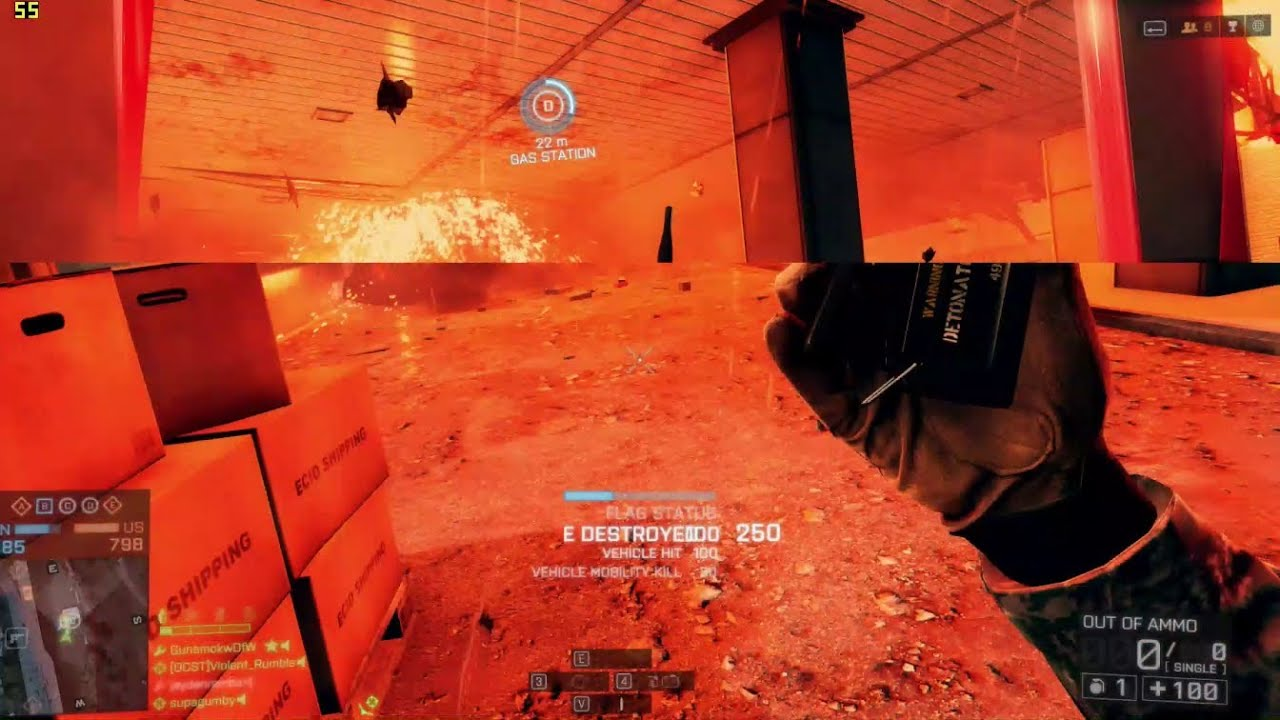
\includegraphics[width=\textwidth]{screen_tearing.jpg}
	\caption{Screen Tearing} \cite{fig:screen_tearing}
\end{figure}

Here you can see that 2 images are displayed at the same time. The top image is the new one that has
not managed to fully render yet and the bottom image is the old one that was being displayed before the
refresh. Remember that we overwrite the old image with the new one when rendering. Because not every pixel
was done rendering when the refresh happened we get the rendered part and the old part displayed at the same time.
This is obviously not optimal and we want to avoid this. So let's move on to the next one.

The next present mode is called
\textit{VK\textunderscore PRESENT\textunderscore MODE\textunderscore FIFO\textunderscore KHR}.
FIFO stands for first in first out. This mode handles the images in a queue. Each fully rendered image
is added to the queue and the image that is at its front is displayed. The
\textit{VK\textunderscore PRESENT\textunderscore MODE\textunderscore FIFO\textunderscore KHR}
only swaps the framebuffers when the vertical blank happens and takes the framebuffer's image that is at the front
of the queue, which avoids the screen tearing effect. The problem with this mode is that if the queue is full,
aka each framebuffer's image is rendered but not displayed yet, the GPU has to wait until the vertical blank happens
to continue rendering, which caps the frame rate to the refresh rate of the monitor. This is called V-Sync and
causes a delay between the rendering and the displaying of the image, but is guaranteed
to be available and has a lower energy consumption than the other modes that have the GPU rendering without a break.
Therefore this mode is the most common mode for mobile devices, but is still widely used for desktop applications.

There is a similar version of the
\textit{VK\textunderscore PRESENT\textunderscore MODE\textunderscore FIFO\textunderscore KHR} mode called \\
\textit{VK\textunderscore PRESENT\textunderscore MODE\textunderscore FIFO\textunderscore RELAXED\textunderscore KHR}.
This mode only differs from the previous mode in the way it handles a empty queue. If the queue is empty, aka no
framebuffer's image is rendered yet, the swapchain will swap the framebuffers immediately and display a teared image. This mode
is used when we have a long rendering time and want to avoid waiting for the queue to be filled.

Finally we have the \\
\textit{VK\textunderscore PRESENT\textunderscore MODE\textunderscore MAILBOX\textunderscore KHR} mode.
This is also the mode that we will be using. This mode is similar to the
\textit{VK\textunderscore PRESENT\textunderscore MODE\textunderscore FIFO\textunderscore KHR} mode,
with the difference that the swapchain will not let the GPU idle when the queue is full. Instead it will
discard the image that is at the front of the queue and start rendering again. This constant rendering
will provide us with the lowest latency but also the highest energy consumption. But that should not
be a problem for our application.

We will simply iterate through the available present modes and return the \\
\textit{VK\textunderscore PRESENT\textunderscore MODE\textunderscore MAILBOX\textunderscore KHR} mode
if it is available. If not we will return the \textit{VK\textunderscore PRESENT\textunderscore MODE\textunderscore FIFO\textunderscore KHR} mode.

\begin{lstlisting}[language=C++]
VkPresentModeKHR SwapChain::chooseSwapPresentMode(const std::vector<VkPresentModeKHR> &availablePresentModes) {
  for (const auto &availablePresentMode : availablePresentModes) {
      if (availablePresentMode == VK_PRESENT_MODE_MAILBOX_KHR)
      return availablePresentMode;
    }

  return VK_PRESENT_MODE_FIFO_KHR;
}
\end{lstlisting}

\subsection{Swapchain Extent}

Like mentioned before we have to choose the extent of the swapchain images. We get the extent
from the devices capabilities. If the width and height of the extent are set to the maximum
value of uint32\_t, we are indicated that the extent is defined in screen coordinates and we
have to get the extent from our windowExtent variable. We then have to clamp
the extent to the minimum and maximum extent that the device supports tho. If the width and height
are not set to the maximum value we can use the extent directly because that tells us that the extent
is already in pixels.

\begin{lstlisting}[language=C++]
VkExtent2D SwapChain::chooseSwapExtent(const VkSurfaceCapabilitiesKHR &capabilities) {
  if (capabilities.currentExtent.width != UINT32_MAX)
    return capabilities.currentExtent;
  else {
    VkExtent2D actualExtent = windowExtent;

    actualExtent.width = std::clamp(actualExtent.width, capabilities.minImageExtent.width, capabilities.maxImageExtent.width);
    actualExtent.height = std::clamp(actualExtent.height, capabilities.minImageExtent.height, capabilities.maxImageExtent.height);

    return actualExtent;
  }
}
\end{lstlisting}

\subsection{Image Count}

The final thing we have to do is to set the min image count of the swapchain. The image count is the amount
of images that the swapchain will contain aka the amount of framebuffers. We will use one more than the
minimum image count that the device supports, for the min image count of the swapchain. This is because
we otherwise would have to wait for the driver to complete internal operations before we can acquire the
next image. Because we increase the min image count
by one we have to check if it is bigger than the max image count. If it is we set the min image count to the
max image count. Except if the max image count of the device is 0, which means that there is no maximum image count.

\begin{lstlisting}[language=C++]
uint32_t imageCount = swapChainSupport.capabilities.minImageCount + 1;
if (swapChainSupport.capabilities.maxImageCount > 0 && imageCount > swapChainSupport.capabilities.maxImageCount)
  imageCount = swapChainSupport.capabilities.maxImageCount;
\end{lstlisting}

\subsection{Swapchain Creation}

Now that we have all the data we need we can create the swapchain. We will populate the
\textit{VkSwapchainCreateInfoKHR} struct with the data we have and additionally set the
image array layers to 1, which is the amount of layers that the image has. This is always
1 unless you are working with stereoscopic 3D applications. We also have to set the image
usage to
\textit{VK\textunderscore IMAGE\textunderscore USAGE\textunderscore COLOR\textunderscore ATTACHMENT\textunderscore BIT},
which means that we will render directly to the image.

\begin{lstlisting}[language=C++]
VkSwapchainCreateInfoKHR createInfo = {};
createInfo.sType = VK_STRUCTURE_TYPE_SWAPCHAIN_CREATE_INFO_KHR;
createInfo.surface = surface;
createInfo.minImageCount = imageCount;
createInfo.imageFormat = surfaceFormat.format;
createInfo.imageColorSpace = surfaceFormat.colorSpace;
createInfo.imageExtent = extent;
createInfo.imageArrayLayers = 1;
createInfo.imageUsage = VK_IMAGE_USAGE_COLOR_ATTACHMENT_BIT;
\end{lstlisting}

But that's not all. We also have to specify the sharing mode of the swapchain. The sharing mode
determines how the images are shared between multiple queue families. We use 2 queue families, the
graphics queue family and the present queue family. Now we have 2 cases. The first case is that the
graphics queue family and the present queue family have the same index. In this case we set the sharing
mode to exclusive. This means that an image is owned by one queue family at a time and has to be
explicitly transferred to the other queue family. In this case the count of queue families and the
queue family indices that are used are not relevant. The second case is that the graphics queue family
and the present queue family have different indices. In this case we set the sharing mode to concurrent.
This means that an image can be used by multiple queue families without explicit ownership transfers.
It is important to note that the queue family indices are relevant in this case, because the swapchain needs
to know what queue families can access the image.

We'll start off by getting the queue family indices from the device. We will then check if the graphics
queue family and the present queue family are different. If they are we set the sharing mode to concurrent
and set the queue family indices and their count. If they are the same we set the sharing mode to exclusive.

\begin{lstlisting}[language=C++]
QueueFamilyIndices indices = device.findQueueFamilies();
if (indices.graphicsFamily != indices.presentFamily) {
  createInfo.imageSharingMode = VK_SHARING_MODE_CONCURRENT;
  createInfo.queueFamilyIndexCount = 2;
  uint32_t queueFamilyIndices[] = {indices.graphicsFamily.value(), indices.presentFamily.value()};
  createInfo.pQueueFamilyIndices = queueFamilyIndices;
} else {
  createInfo.imageSharingMode = VK_SHARING_MODE_EXCLUSIVE;
}
\end{lstlisting}

We're still not done yet! We also have to specify if and what kind of transformation we want
to apply to the images. For example we might want to flip or rotate the image. We don't want
anything to happen to the image so we set the pre transform to the current transform. We get
the current transform from the swapchain support details capabilities. We also have to specify
the composite alpha. The composite alpha is used to blend the window with other windows in the
system. We want to ignore the alpha channel so we set the composite alpha to the opaque bit.
Finally we specify our present mode, the clipped flag and the old swapchain. The clipped flag
indicates that we don't need the pixels that are obscured by other windows. If you need the
pixels to predict future frames you can set the clipped flag to false but we will keep it true.
The old swapchain is used to create a new swapchain from an old one. We will set it to
\textit{VK\textunderscore NULL\textunderscore HANDLE}, but will come back to this later.

\begin{lstlisting}[language=C++]
createInfo.preTransform = swapChainSupport.capabilities.currentTransform;
createInfo.compositeAlpha = VK_COMPOSITE_ALPHA_OPAQUE_BIT_KHR;
createInfo.presentMode = presentMode;
createInfo.clipped = VK_TRUE;
createInfo.oldSwapchain = VK_NULL_HANDLE;
\end{lstlisting}

Now that we have the create info struct we can create the swapchain with the \textit{vkCreateSwapchainKHR}
function, that takes the device, the create info struct, a custom allocator and a pointer to the swapchain
variable that we also have to add to our header. We again will check for an error and throw an runtime
error if the creation was not successful.

\begin{lstlisting}[language=C++]
if (vkCreateSwapchainKHR(device, &createInfo, nullptr, &swapChain) != VK_SUCCESS)
  throw std::runtime_error("Failed to create swap chain!");
\end{lstlisting}

After the creation of the swapchain we need to store the images of the swapchain. We can get the images
with the \textit{vkGetSwapchainImagesKHR} function. We have to specify the device, the swapchain, a pointer
to the image count and a pointer to the images. We will store the images in the \textit{swapChainImages}
vector. Then we should also create a variable for the image format and the extent of the swapchain images
and store them in the class.

\begin{lstlisting}[language=C++]
//swapchain.hpp
private:
  ...
  VkSwapchainKHR swapChain;
  VkFormat swapChainImageFormat;
  VkExtent2D swapChainExtent;
\end{lstlisting}

\begin{lstlisting}[language=C++]
vkGetSwapchainImagesKHR(device, swapChain, &imageCount, nullptr);
swapChainImages.resize(imageCount);
vkGetSwapchainImagesKHR(device, swapChain, &imageCount, swapChainImages.data());

swapChainImageFormat = surfaceFormat.format;
swapChainExtent = extent;
\end{lstlisting}

If you ask yourself why we have to get the image count first and then resize the vector, it is because
we have only defined the minimum image count of the swapchain in the imageCount variable. The actual
image count could be different.

Now we have to make sure that the swapchain is destroyed in the destructor. We can do this by calling
the \textit{vkDestroySwapchainKHR} function.

\begin{lstlisting}[language=C++]
SwapChain::~SwapChain() {
  vkDestroySwapchainKHR(device, swapChain, nullptr);
}
\end{lstlisting}

\section{Pipeline Creation}

Let's go and create our first Vulkan pipeline. We will keep it simple and ignore
buffers and perspective projection for now.


\printbibliography[
	heading=bibintoc, title={Bibliography}
]

\listoffigures

\end{document}
